\documentclass[a4paper,9pt]{article}
%\documentclass{aa}
%\pgfplotsset{compat=1.12}
\usepackage{conference}
\usepackage{latexsym}
\usepackage[perpage,symbol*]{footmisc}
%\usepackage[utf8]{inputenc}
\usepackage[utf8x]{inputenc}
\usepackage{textcomp}
\usepackage[english]{babel}
\usepackage{amssymb,amsfonts,amsmath}
\usepackage{xcolor}

%\usepackage{graphicx}
%\usepackage{pstricks,pst-node}             % Pstricks
\usepackage{tikz}
\usepackage{tikz-3dplot}
\usepackage{pgfplots}
\usepackage{pgfplotstable}

\usepackage{cite}
\usepackage{hyperref}
\usepackage[varg]{txfonts}
\usepackage{booktabs}       % professional-quality tables
%\usepackage[letterpaper, landscape, lmargin=0.25in, rmargin=1.25in]{geometry}
\usepackage{tabularx}
\usepackage{enumerate}
%\usepackage{enumitem}
\usepackage{multicol}
% \usepackage{ifpdf}

% \usetikzlibrary{shapes}
% \usepackage[left=0.1cm, right=0.1cm, top=0.1cm, bottom=0.1cm]{geometry}
% \usepackage[ansinew]{inputenc}           % Input
\usepackage[T1]{fontenc}                   % Font encoding
% \usepackage{cmbright}                    % Font style
%\usepackage[nohead,margin=0mm]{geometry}  % Page & margins

%%%%%%
%%%%%%

\usetikzlibrary{patterns,arrows,calc,angles,positioning,intersections,through,quotes,decorations.markings}
\usepackage{tkz-euclide}
\usetkzobj{all}

\newcommand\RectTri[4][thick,green!50!black,text=black]{%
\coordinate [label=left:$C$] (C) at #2;
\coordinate [label=below right:$B$] (B) at #3;
\coordinate (aux) at ($ #2 ! 1 ! 90:#3 $);
\coordinate [label=above:$A$] (A) at ($ #2 !#4!(aux) $);

\coordinate (perp) at ($(A)!(C)!(B)$);
\draw[purple!70!black,thick,dashed] (C) -- (perp);

\draw[#1] 
  (C) -- 
  node[auto] {$\sqrt{a''}$} (A) -- 
  node[auto] {$\sqrt{a}$} (B) --
  node[auto] {$\sqrt{a'}$} 
  (C)
  pic ["$\theta$",draw,red,thick,angle radius=1cm] {angle = C--A--B} 
  pic ["$\alpha$",draw,cyan,thick,angle radius=1cm] {angle = B--C--perp}
  pic ["$\beta$",draw,orange!70!black,thick,angle radius=1cm] {angle = A--B--C}
  pic ["$\beta$",draw,orange!70!black,thick,angle radius=1cm] {angle = perp--C--A};
}

\tikzset{
mydot/.style={
  fill,
  circle,
  inner sep=1.5pt
  }
}

%%%%%%%
%%%%%%%
%%%%%%%

%% Begin of Watermark feature
%\usepackage[printwatermark]{xwatermark}
%\usepackage{xcolor}
%\newwatermark[allpages,color=red!50,angle=60,scale=6,xpos=0,ypos=0]{DRAFT}
%\newwatermark[allpages,color=red!20,angle=60,scale=2,xpos=0,ypos=0]{For Peer Review}
%% End of Watermark feature

%\pagenumbering{gobble}

\title{Science unification and Permanent Cosmology}

\author{F. M. Sanchez \thanks{Retired Prof. of Physics, University of Paris 11, Orsay, France, \href{mailto:hol137@yahoo.fr}{hol137@yahoo.fr}} 
   %%\\ email \href{mailto:hol137@yahoo.fr}{hol137@yahoo.fr}  	  
   \and M. H. Grosmann \thanks{Retired Prof. of Physics, University of Strasbourg, France, \href{mailto:michelgrosmann@me.com}{michelgrosmann@me.com}}
   %%\\ email \href{mailto:michelgrosmann@me.com}{michelgrosmann@me.com} 
   \and R. Veysseyre \thanks{Retired Agregee de mathematiques et professeur honoraire \`a l'Ecole centrale de Paris, France, \href{mailto:renee.veysseyre@normalsup.org}{renee.veysseyre@normalsup.org}}
   %%\\ email \href{mailto:renee.veysseyre@normalsup.org}{renee.veysseyre@normalsup.org} 
   \and D. Weigel  \thanks{Retired Prof of Cristallography, University of Paris 6, Paris, France, \href{mailto:dominiqueweigel18@gmail.com}{dominiqueweigel18@gmail.com}} 
   %%\\ email \href{mailto:dominiqueweigel118@gmail.com}{dominiqueweigel118@gmail.com} 
   \and L. Gueroult \thanks{Retired PhD instructor in Holography at ENS, Physics department A2, Cachan, France, \href{mailto:lgueroult@hotmail.com}{lgueroult@hotmail.com}}
   %%\\ email \href{mailto:lgueroult@hotmail.com}{lgueroult@hotmail.com}
   }

\begin{document}
\setcounter{page}{1}

\maketitle

\begin{abstract}
The hypothesis that the Cosmos is a computer leads to a reunification of Arithmetics and Physics, through a systematic optimisation and symbolic rationalisation process, the later being a kind of renormalisation, in the sense that this minimizes the number of parameters. The $20 = 16 + 4$ main parameters of particle physics are so defined to ppb precision ($10^{-9}$). A computer analysis of the 4 coupling constant confirms the BIPM $G $value in the 10 ppm domain, showing that the official value of $G$ is erroneous by $7.5 \sigma$. The extrapolation of the operational definition of the Euler-Mascheroni constant $e$ leads to a relation characterizinging the electric constant $a$. The $\pi$ symbolic rationalisation rehabilitates the Wyler's theory and specifies the Koide Fermion formula in the ppb domain. The Eddington's equation is interpreted as the kernel of an holographic process from 16D to 4D space, with a connexion in the 10D superstring space of the Topological Axis. The computer indicates an holographic relation tying the Wyler term with the proton, Hydrogen and Nambu masses, leading to a characterization of the Monster group tying the canonical dimensions 16 and 24, both central in the string theory and the Topological Axis. The analysis shows that the 26 sporadic groups are involved, with special importance of the Matthieu family, leading to a confirmation that the Higgs boson is a central particle, associated to the subperfect number 495, which is tightly connected with the Eddington's equation throught the Lucas-Lehmer generator. The Permanent Oscillatory Cosmology is confirmed by 225 formulas for the invariant Hubble radius, whose 19 are ppb precise. 
\end{abstract}


% keywords can be removed
\keywords{Quantum Physics \and Quantum Gravity \and String Theory \and Number theory \and Cosmology \and Holographic \and Holic Principle \and Crystallography}



\label{sec:headings}

\tableofcontents




\section{Introduction}
  
    From Hirzebruch's work \cite{Hirzebruch}, which revolutionized geometry and topology, Sir Michael Atiyah, Raoul Bott \cite{Bott} and Isadore Singer \cite{Singer} introduced the index theory, acclaimed by theoretical physicists \cite{Alvarez}. Following this path, on the advice of the physicist Gerard t'Hooft, Atiyah looked for the determination of the electrical constant $a \approx 137.035999085(21)$ \cite{Atiyah}.
    
    
    At the 2018 Heidelbergh Laureate Forum, he showed that the extrapolation of the Euler formula  $e^{2i\pi} = 1$ to the quaternions leads to the 'Atiyah constant' $\Gamma = \gamma a/\pi $. Meanwhile, he rehabilitated the Eddington \cite{Eddington} bare electrical constant, the prime number 137, and announced that the resolution of the Riemann conjecture appears as a "bonus". Moreover, the four forces would be connected to the four principal algebras, whose the octonion non-associative one would be tied to the gravitational constant $G$ in a future work \cite{Atiyah}. 
    
    
Indeed, it seems that Eddington was really ahead of his time, according to Salingaros \cite {Salingaros} :\textit{Eddington anticipated results of current interest. He discovered the Majorana spinors, and was responsible for the standard $\gamma^5$ notation as well as the notion of chirality. Furthermore, Eddington defined Clifford algebras in eight and nine dimensions which are now appearing in grand unified gauge and supersymmetric theories. A point which Eddington cleared up, yet is still misunderstood, is that the Dirac algebra corresponds to a five-dimensional base space}.


       






\section{The scope and method}
   Quite independently, the $G$ value was tied to the invariant Hubble radius $R$ in the \textit {Coherent Cosmology}. A computer analysis has shown that it is confirmed in the ppb domain ($10^{-9}$) by simple formula involving the Atiyah constant \cite{Sanchez}. The aim of this article is to confirm the above \textit {physics-arithmetic unification}.
   
   Our main hypothesis is that \textit{both} mathematics and physics standard model are widely incomplete, and that the so far unexplained measured a-dimensional constants (see Table \ref{tab:1:table1}) can be used as a guide for the overall arithmetics unification. Recall that the search for correlations between measurements is the heart of the scientific method, as the history shows, through Dalton, Proust, Balmer, Mendeleyev, Mandel... In particular, it was already shown that the Atiyah constant enters the core of Coherent Cosmology, the Topological Axis (Fig. \ref{tab:9:table9}), both in connection with the Higgs boson and the galaxy group radius, a crucial cosmic distance \cite{Sanchez}. The pertinent data is completed by physical and cosmic constants in Tables \ref{tab:2:table2} and \ref{tab:3:table3}.
   
   
   In conformity with this physics-mathematics unification idea, the Table \ref{tab:1:table1} mixes physical adimensional constants \cite{Tanabashi} with pure mathematical constants. But among the latter an important distinction is made. Only the whole numbers are considered really exact. For instance, the Archimedes constant $\pi$ is referred only as 'exact', meaning one can uses it in a computer calculation, only if one defines an imprecision domain. This is known in computer science as the floating problem: when dealing with numbers different from whole  numbers, the equality is excluded, only the sign $\approx$ is valid. From this kind of argument, the Cosmos vastness has been justified by quantinuum holography (meaning quasi-continuous), where the whole large numbers of Lucas-Mersenne \cite{Bastin} and Eddington \cite{Eddington} are central \cite{Sanchez}.
      
      
   In particular, the fact that the Muon-Electron mass ratio is measured to 10 ppb, while nobody knows the role of Muon in Nature, is very intriguing. We show here that this permits to definitely validate the empiric, but dramatically simple, Koide fermion formula, connected with a rehabilitated Wyler's theory through $\pi$ rationalization process. 
   
   
   While the Atiyah's work does not seem to give the $a$ value, nor the Riemann conjecture solution, he suggested \cite{Atiyah1} \textit{there is a bridge between the octonion algebra and the sporadic groups} : \textit {the real theory which we would like to get to should include gravity with all those theories in such a way that gravity is seen as a consequence of the octonions and the exceptional groups. It will be hard, because we know the octonions are hard, but when you have found it, it should be a beautiful theory and it should be unique}. 
   
   
   
   This article will confirm this Atiyah's prediction, connecting, through cosmology, these two apparently separated mathematical domains, octonions and sporadic groups.
   
   
   
   Note that the Topological Axis (Fig. \ref{tab:9:table9}) shows clearly the eight-fold Bott periodicity, typical of octonion algebra, and that Coherent Cosmology involves the sporadic groups \cite{Sanchez}. In section 6 this connection will be strengthened by a study of the Ramanujan number, tied to the modular function and the Monster group, the largest of the 26 sporadic ones \cite{Conway} \cite{Borcherds}. In particular, the 20 groups of the Monster family were already connected to the computing canonic number $a^a$ \cite{Sanchez}. The section 7 shows the unambigous connection of this term $a^a$ with the Lucas-Lehmer generator, the Topologic Axis function and the weak boson masses.  
   
   
   This end of this article will show also the unexpected liaison between the \textcolor{red}{Topologcal} Axis and the Periodic table of elements, as well a multi-dimensional crystallography.
   
   
   \subsection{The warning of Feynman}
   Feynman declared\footnote{\textcolor{red}{\textbf{do not copy} without citing, book reference please}}: ... \textit{That summarizes all of the problems associated with Quantum Electrodynamics. The most beautiful one is the coupling constant, 137 point and so on, and all good theoretical physicists put that up on their wall and worry about it. There is at the present time no idea of any utility for getting at that number. There have been from time to time suggestions, but they didn't turn out to be useful. They would predict that the number was exactly 137, when it — well. The first idea was conceived by Eddington, and experiments were very crude in those days and the number was very close to 136, so he proved by pure logic that it had to be 136. Then it turned out that experiment showed that it was a little off, and it was nearer 137. So he found a slight error in its logic and proved with pure logic that it had to be exactly the integer 137. It's not the integer. It's 137 point oh three six oh.
  Every once in a while someone comes out and they find out that if they combine pi's and e's and 2's and 5's with the right powers and square roots that you can make that number.
  It seems to be a fact that's not fully appreciated by people that play with arithmetic — that you'd be surprised how many numbers one can make by playing with pi's and 2's and 5's and so on — and if you haven't anything to guide you except the answer, one can always make it come out even to several decimal places by a suitable jiggling about. It's surprising how close one can make an arbitrary number by playing around with nice numbers like pi and e. It's, and therefore throughout the history of physics, there — paper after paper of people who have noticed that certain specific combinations give answers which are very close in several decimal places to experiment disagrees with it — so it doesn't mean anything.}
  
Feynman simply forgets here the science history. Looking for whole values in experimental data was \textit{determinant} for Dalton, Balmer, Mendeleyev, opening respectively chemistry, atomic physics, nuclear physics and biology.
   
   
 \subsection{The Eddington's 137 and the electroweak coupling constant}

Eddington predicted the importance of the $N_{16} = 136$ elements of a symmetrical matrix 16 x 16, giving 137 by adding unity, whose pertinence is confirmed by the very precisely (0.1 ppm) measured electroweak coupling (inverse) factor 

\begin{equation}
a_w = (2\times137 \Gamma)^3
\end{equation}
 
Atiyah presented this number by the form $137 = 2^0 + 2^3 + 2^7$. Moreover, this additive unity is clearly tied to the Combinatorial Hierarchy \cite{Bastin}, based on the Catalan-Mersenne series starting with 3, because $N_4 = 10 = 3 + 7$ and $3+7 + 127 = 137 = N_{16} + 1$. The following term $N_{32}  = 528$ cannot be compared with the huge Lucas-Mersenne Large Number $2^{127}- 1$, so it is the last term of the Hierarchy.


Note that Atiyah considered the suite of the characteristic numbers of three of the four main algebra: 0 (real numbers), 3 (quaternions), 7 (octonions). Adding the unity of the complex numper, he would have obtained 139, which is the entire pat of $a_0$ 

This Lucas number appears in the ppb precise formula of Table \ref{tab:3:table3}, in liaison with 137. Moreover $32^2 - N_{32} =  496$ is the above dimension of the superstring gauge group SO(32), and \textit {the third perfect number}, see below the paramount importance of this fact, unrecognized up to this day.  
   
   
   

 
 
 
 
 
 
 
 
 
 
 
 
 
 
 
 
 \section {The remarkable properties of $e$ }
 
 It seems that the following properties of $e$ were not emphatised 
  
 \subsection {The musical properties of $e^2$}
 
 The Euler series $e \approx (1+1/n)^n$ converges rather slowy. More rapid is the series:
 
 \begin{equation}
e^2 \approx (3/2)^5 \approx (4/3)^7 \approx (5/4)^9 \approx (6/5)^11 ...
\end{equation}
 
 connecting the main musical intervals
 
  \subsection {The symbolic rationalisation of $e$ }
 
 The fractional development of $e$ shows unambigously the central gravitational parameter, tied to the Lucas number \cite{Sanchez}  $p_G = P/2^{127/2}$ 
 
 \begin{equation}
e : 2,7/5, 3\sqrt{p_G}
\end{equation}
 
This was discovered starting from the approximation $e\approx 19/7$, tied to the Archimedes approximation $\pi_{Arch}= 22/7$ and the following property of the first terms of the Combinational Hierarchy  : $2^7/3 \approx \sqrt p$. 


\textit{This confirms our value of $G$ in the ppm domain}.


 
 
 \subsection{The Planck law connection with the Bernouilli function}

A computer analysis shows that $a$ is tied with two central constants of the Planck law, whose kernel is the Bernouilli fonction, $x/(1-e^{-x})$, \textit {central in the Atiyah's work} \cite{Atiyah}. These constants are the reduced Wien displacement constant $w$ and the number of photons $16\pi \zeta(3)$ in a volume $\lambda^3$, where $\lambda = hc/kT $. This defines a length $l_{ph} = \lambda/(16\pi \zeta(3))^{1/3}$ corresponding to one photon by volume $l_{ph}^3$:

\begin{equation}
(16\pi\zeta(3))^3/w^4 = \lambda^5l_{Wien}^4/l_{ph}^9 \approx \pi_a^3a    \Rightarrow     \pi_a: 3;7;16;17p_an/p
\end{equation}

This seems to imply the 9D space of superstring theory. 



\subsection {The Trigonometric Formula}
From the proximity of $a + 2\pi$ with the Planck law term $e^w$, it was investigated if $a$ was a trigonometric line. Indeed 
 
\begin{equation}
\cos{a} = 1/e_a ~~~~~~~~  e_a : 2, 7/5, ee_a \sqrt{dn/2\pi} 
\end{equation}

So, it is confirmed that Nature uses approximations of the optimal basis $e$, whose operational definition plays a central role in the following.

 
 
 
 
  \subsection{The holographic connection with 10D and 11D spaces}
 
One notes that the central term of the Planck law connects with the Topological axis for $d = 10$:

\begin{equation}
 e^w \approx f(10)      
\end{equation}


\begin{equation}
 p_G^2 + f(10)^2 \approx p_{hol}^2      
\end{equation}

where $p_{hol}$ is the holographical spherical trm in the hydrogen atom: 

\begin{equation}
\pi p_{hol}^2 \approx (4\pi/3) (r_H/\lambdabar_e)^3 = (4\pi/3) (aH/p)^3   
\end{equation}

The superstring and supergravity theories implies the spaces of dimensions 10 and 11, represented in the topologcal Axis by the terms $f(10)\approx e^w$ and $f(11)$ which corresponds to the Pions and KaonsUsing instead the 11D term, one gets:

\begin{equation}
 p_G^2 + f(11)^2 \approx f(\sqrt{aH/p})      
\end{equation}

confirming the holographic character of the topological function.
 
 
 
 
 
 
 
 
 
 
 



     
   
   \subsection{The computational signifiance of $a$}
   
         The present standard model of physics is incomplete, since 30 or so parameters are not calculated from the theory and so appear as 'free parameters'. As these parameters are not recognized by mathematicians, this would mean either that they are arbitrary, or they belong to an unknown domain of mathematics. 
         
         
         Now it was observed that these parameters are tightly interconnected, in a manner that favors life, a phenomenon called 'anthropic fine-tuning'. There is again two possibilities : either there would exist a multiplicity of different universes, or the present mathematics is incomplete.
         
         
         The message of Atiyah is clearly that the search must focus on an extension of present mathematics.
         
         
         In fact, the Topological Axis shows an \textit {objective} fine-tuning, independant of biological issues (Fig. \ref{tab:9:table9}), but the associated function $exp(2^{d/4})$ seems to be unknown in present mathematical theories.
   
         
         
         Our main hypothesis is that \textit {the Cosmos is a computer using these parameters as optimal calculation basis},
         in particular the electric constant $a$ and the proton-electron mass ratio $p$.
         
         
        So one may expect that the term $a^a$ would be related to $p$, in a manner that recalls the definition of the natural basis $e$:
         
\begin{equation}
\frac{d}{de}(e^{1/e}) = 0 
\end{equation}

   Indeed one observes that:
   
 \begin{equation}
 a^{a/p} \approx e^{1/e} 
 \end{equation}
 
 \begin{equation}
 (a^2)^{a^3} \approx (p-1/2)^{(p-1/2)^2} \approx e^{\pi_4^3}
\end{equation}

Making the substitution $e \to i$, one considers the term $i^{\pi/i} = e^{\pi^2/2} = a_0$ which shows direct connection with $a$
   
\begin{equation}
\sqrt{a_0} = i^{\pi/2i} \approx \sqrt a + d_e/ \sqrt a ~~~~~\rightarrow \pi_{a_0} : 3, 7, 16, -284
\end{equation}
 
Note that $\sqrt 284$ is close to $f(1) = g(1)$, the essential term of the Topological Axis. Quite independently, Hans de Vries \cite{deVries} gave a similar formula by assuming other terms in the development, but without mention of the $\pi$ rationalization. 











 \section {The remarkable properties of $\pi$ }
 
 The powers of $\pi$ appear in the even Riemann series, suggesting that $\pi$ must be seen as a computation basis.  
   
\subsection{The neutron factor in $\pi_4$}

Atiyah insisted on a parallel between the Archimedes constant $\pi$, suggesting that $a$ would be a renormalization of $\pi$ , and he introduced his constant $\Gamma$ such that:

\begin{equation}
a/\pi \approx \Gamma/\gamma
\end{equation}

and he remarked that the couple $137,a$ shows $a^2 - 137^2 \approx \pi^2$, so we note:

\begin{equation}
a^2 - 137^2 = \pi_{a,137}^2
\end{equation}

But, \textit {in the hypothesis that the cosmos is a computer}, the cosmos cannot use the mathematical Archimedes constant $\pi$, which is an idealization, \textit {otherwise any time calculation would be infinite}. Its fractional decomposition is an unresolved problem, but the first terms are : $3, 7, 16, -293.634$, where the forth term, highly singular, is so close (3 ppm) to $1 + n/2\pi$, where $n$ is the neutron/electron mass ratio.

\begin{equation}
\pi : 3, 7, 16, -\pi_4 ~~~~~~~   \pi_4 \approx (1+n/2\pi)
\end{equation}






 \subsection {The couple $137, a$ and the symbolic rationalisation of $\pi$ }
This leads to consider the equation:

\begin{equation}
 (a/\pi_a)^2 - (137/\pi_{137})^2 = 1
\end{equation}  

Starting with $\pi_a = \pi$, this leads to the following development of $\pi_{137} : 3,7,16,5\times 137/d_e$, where $d_e$ is the excess electron magnetic moment, tightly tied to $\sqrt{a}$ in quantum electrodynamics. Adopting precisely this value, this induces a slighty variation of the development of $\pi_a$, characteristic of the isospin symmetry neutron-Hydrogen, leading to a value compatible with experiment:

\begin{equation}
\pi_a : 3, 7, 16, -(1+ \sqrt{nH}/2\pi) ~~~~ \rightarrow a \approx 137.035999095343
\end{equation}

\textit{As predicted (Holic Principle, Sanchez 1995), it is now proven that the physical constants are tied to rational approximations of $\pi$: this could be ultimate signification of the renormalisation. Indeed the two process share a common goal: to get rid of infinities.}
%Note that with the well-known approximation $\pi_{137} = 355/113$, corresponding to the fractionnal limited series $3,7,16$ %one finds that $\pi_a$ corresponds to the series $3,7,16,-3\sqrt{137a}/2$, which in turn favors for $\pi_1$ the series  %$3,7,16, 1-5a$ 
 
 
 


\subsection{The auto-holic property of $\pi$}

Nobody seems to have noted the 2D-3D holic following property:

 \begin{equation}
\pi^2 \approx (\pi - 1 )^3 
 \end{equation}
 
Inserting $\pi$ and $\pi-1$ in the correlation program, the computer indicates immediately

 \begin{equation}
\sqrt a /8 \approx \pi/(\pi-1) \approx (\pi - 1)^2/\pi 
 \end{equation}

implying

 \begin{equation}
u = \pi + 1/\pi \approx \sqrt a /8d_e^2 + 2
 \end{equation}

with the symmetric term $v = 2 - \sqrt a /8 = 4 - u $, one notes:

\begin{equation}
uv \approx \tau / 9 \mu
\end{equation}

precise to 6 ppm. This connects again with the Topological function : $f(6) \approx \tau / \mu$. 

With $u_a = \sqrt a /8d_e^2 + 2$, one notes:

\begin{equation}
u_a (4-u_a)^2 \approx (2 \times 3^3 )^{1/\pi a}
 \end{equation}

precise to 30 ppb, showing that \textit{the cosmos uses the approximation $e^4\approx 2\times 3^3$}. Using the above first musical term 
$e^2\approx (3/2)^5 $ one gets $3^7/2^11 \approx 1$, which is the classical apotome interval. Moreover $3^11 - 2^7 = 139 = E(a_0) = 2^0 + 2^1 +2^3 + 2^7$, which is the sum corresponding to the four division algebra, corresponding to the dimensions $1,2,4,8$, with the reduced numbers $0,1,3,7$. Atiyah noted only the reduced sum : $2^0 + 2^1 +2^3 + 2^7 = 137$. 














\subsection{The Rehabilitation of Wyler's theory}

Atiyah did not consider this computation point of view, but he insisted on the analogy of his procedure with that of Archimedes for the calculus of $\pi$ \cite{Atiyah}.

\subsubsection {The Wyler formula}

In the famous Wyler formula \cite{Wyler} \cite{oeis1}

\begin{equation}
\bigg(3\sqrt{\frac{a}{4}} \bigg)^8 = 120 \times \pi_W^{11}
\end{equation}


implicitly tied to the \emph{11D supergravity space}, the development of  $\pi_W$ shows an analogy with the natural one, except for the insertion of \textit {the singular prime 163} :

\begin{equation}
\pi_W : 3, 7, 16,- 163/2, -(1+n/4\pi) ~~~~\Rightarrow ~~~~    a \approx 137.03599908399
\end{equation}


This number 163 is the last of the Heegner-Stark numbers: 163, 67, 43, 19, 11, 7, 3, 2 \cite{Stark}. 


Moreover, according to Atiyah \cite{Atiyah1}, an approximation of $\pi$ appears directly in $(a^2-137^2)^{1/2} = \pi_{a,137} : 3, 7, 10, a_s$, , where the forth term is very close to the inverse strong coupling constant $1/a_s \approx 0.1179(10)$ \cite{Tanabashi}. 




\subsubsection {The Lenz-Wyler formula}

The proton-electron mass ratio of Wyler \cite{Wyler} is the simple formula, which was published by Lenz in the shortest of all articles, only one line: 

\begin{equation}
 p_W = 6\pi^5    
\end{equation}

which is \textit {the product of the area of a cube of side $\pi$ with its volume}. As seen above this formula is central in the connexion betxeen $a$ and $\Phi$. There is a direct coonexion with the Eddington's equation, as explained below. 

\subsection {The Koide-Wyler ppb relation}

While $\mu$ is measured to 10 ppb, $\tau$ is rather badly measured. The Koide relation \cite{Koide}, always unexplained, has shown correct predictability for the $\tau$ mass, proving \textit{the present standard particle theory is badly insufficient}. This relation writes in the most symmetrical way connecting with the above Wyler formula, in the following \textit{ppb formula, which confirms the specified ppb value}: $\mu = (Fa/\sqrt{pH})^{1/2}$\cite{Sanchez}.


\begin{equation}
(1 + \mu + \tau)/2 = (1 + \sqrt{\mu} + \sqrt{\tau})^2/3 = p_K \approx 6\pi_K^5 (1+(\mu / \tau)^2) ~~~~\pi_K: 3,7,16,-(2\times 137)^{2/3}
\end{equation}

The fermions Mu and Tau masses are complete mystery in the standard model. However, Eddington predicted the tau fermion, 35 years before its fascinating discovery, calling it « heavy Mesotron », with a right order prediction of its mass \cite{Eddington}.  This was very surprising because the Eddington theory appeared so obscure, and was fully rejected.







\subsubsection {The Lenz-Wyler monster group connection}

A research on computer looking for an holographic relation, of type $3X^2 = Y^3$, between the terms $a, p_W, p$ and $H$ leads to the following 61 ppm relation, involving the canonic dimensions 16 and 24, and connecting with the monster group order to 100 ppm, which in turn connects with a combinaison of basic elements, to 1.5 ppm:

\begin{equation}
3 (p_W H/p)^{16} \approx (H^2/p_W \sqrt a )^{24} \approx O_M / 16 \approx (a \mu n K W/2 \Pi_0)^4
\end{equation}

The corresponding precise values for the involved three values for $\pi$ shows up characteristic formal fractional developments. 



\subsection{The computational confirmation of the 4 coupling constants}
When mixing the four coupling constants (Table 1), defined previously in the ppb range \cite{Sanchez}, the computer indicates immediately the following correlation involving $\pi^{1/\pi}$, with an exponent close to $\pi_4 - 1$:  

\begin{equation}
(Pa_s^2)^6 \approx (a_w/a)^{31/2} \approx \pi^{\pi_4 - 1} \approx (lna)^{210} \approx a_s^{H/\sqrt a}
\end{equation}

This correlation is precise in the ppm range. The $210$ exponent is clearly the holic one  \cite{Sanchez}, but the exponent $31/2$ is not yet understood. Another correlation is revealed by the computer, without $a_s$, with exponents directly tied to the Combinational Hierarchy \cite{Bastin}:
$10 = 3+7$ and $134 = 127+7$:

\begin{equation}
P^{10} \approx a_w^7 \sqrt a^{134}
\end{equation}

Rearranging the terms, and eliminating $a_w$ through $ P/a_w \sqrt a \approx n^3 $:

\begin{equation}
P n^7 \approx a^{127/6}
\end{equation}

This suggests to look for $P^{1/7}$, which is close to $(2\pi)^4$. And the miracle of rationalisation works again, with the Lenz-Wyler formula (recalled below) : $p_W = 6\pi^5$, leading to a  $P$ value precision in the ppm range:

\begin{equation}
P \approx (2\pi_P)^{28}      ~~~~~~  \rightarrow ~~~~ : \pi_P : 3, 2\times 137p_W/pH 
\end{equation}


\textit{The $G$ value is again confirmed by optimising correlations, so the the 180 ppm-distant official value of $G$ confirms to be erroneous by $7.5 \sigma$}.
   













   
   
  \section{The computational signifiance of the golden ratio} 
  
  The golden ratio $\Phi = (1+\sqrt 5)/2$ shows singular arithmetical and geometrical properties. The connections with $a$, the whole value $E(p) = 1836$ and the computational term $e^{1/e}$ are direct :
  
\begin{equation}
\Phi^a \approx (a^{1/a})^{1836 + 1/\Phi} \approx (e^{1/e})^{p_G \sqrt{nH}/a^2}
\end{equation}    
  
Moreover:

\begin{equation}
a^a \approx (e^e)^{(2\pi_{a,e})^3}     ~~~~ \rightarrow   \pi_{a,e} : 3, 7, 15 + 1/\Phi
\end{equation}  
   
Looking for a direct relation tying $a$ and $\Phi$, one remarks that: 

\begin{equation}
a \approx 20 ~ \Phi^4
\end{equation}  
   
Again, a rationalisation for $\phi$ isnecessary. It will be specified in the next section.


 







   
\subsection{The Eddington's large number and the Monster group order}

The Eddington's large number enters the Coherent Cosmology, beeing the equivalent number of neutrons in the fraction 3/10 of the critical mass \cite{Sanchez}. Note that this \textit{trivial} gravitational factor 3/10 is currently associated to a "dark energy". There is a direct connection with the Monster group order $O_M$:

\begin{equation}
N_{Ed} = 136 \times 2^{256} \approx (3/10) P^4/H^2 n \approx O_M P \times 6 \times 136\times 137/a
\end{equation} 

implying the above canonical factor $a/20$. The analysis leads to:
 
 \begin{equation}
a^2/137 \approx 20 ~ ( p_{W,\Phi}\Phi/p)^4   ~~~~~ \Rightarrow  p_{W,\Phi} = 6\pi_{\Phi}^5  ~~~~ \pi_{\Phi} : 3,7,16,a_s^2\tau/\mu  
\end{equation}  
 
implying again the Lenz-Wyler formula $p_W$.


\subsection{The liaisons between $a$, the weak mixing angle and the golden ratio}

Thus, the physical parameters would be mathematical constants of an unknown arithmetical domain. So, their « fine-tunings» is not due to chance in a \textit {disparate Multiverse}, but are of mathematical origin in a single Cosmos, which is unifying \textit{coherent universes}. One main observation of Coherent Cosmology is that, with unit length the Hydrogen radius $r_H$, the Cosmos volume involves $a^a$, confirming that \textit{$a$ is an optimal computation base}  \cite{Sanchez}:

\begin{equation}
    (4\pi /3) (R_C/r_H)^3 \approx a^a/\pi \approx (1/ln2)^{\sqrt{pH}} \approx (13/3)^{p/4} \approx (1/sin^2\theta)^{n/4} 
\end{equation}

where $p$, $H$ and $n$ are respectively the proton-electron, hydrogen-electron and neutron-electron mass ratios, and 13/3 the fraction associated to the decomposition 16 = 13 + 3 \cite{Sanchez1}. This corresponds to the value $sin^2\theta \approx 0.231235$, compatible with the measured weak mixing angle 0.21322(4) \cite{Tanabashi}. Note that the presence of $\ln{2}$ involves information theory \cite{Shannon}. 


The \textit {effective} mixing angle 0.21355(4) \cite{Tanabashi} is compatible with $\ln^2{\Phi} \approx 0.2315648$. It appears unambigously in:

\begin{equation}
a_0 = i^{\pi/i} \approx \pi_{\Phi}^{1/(ln\Phi) ^2} ~~~~\rightarrow : \pi_{\Phi}: 3; e^2; -3\sqrt{p/n}/H
\end{equation}

such a so special fractional development cannot be due to chance. 


Moreover:

\begin{equation}
\Phi^{\pi^2}/\pi^2 \approx \sqrt{137}
\end{equation}

For confirmation of the pertinence of the term $1/ln\Phi$, the correlation with the above main series is positive:

\begin{equation}
\sqrt{1/ln\Phi} \approx \Pi_0 K_0/Z
\end{equation}

an expression involving only neutral particles.



\textit{This confirms the importance of the Golden number, and its associated effective weak mixing angle.}













 
 \section{The connections with the sporadic groups }

\subsection{The Monster group} 
 
Note that, very precisely:

\begin{equation}
O_M \approx (F/aa_s)^{20} \approx (a-136) ~ 495^{20} \approx (e^w)^25 \approx e^{e\times 137/3} \approx \tau^{137/9}
\end{equation}

showing that the lepton $\tau \ e^{3e}$, which seems so useless in standard physics is very important in the correlation process 

\begin{equation}
lnO_M /lnlnlnlnO_M\approx 2\times 137
\end{equation}

This must be tied to the liaison of the Monster group with 16D space, which is central in the topological axis:

\begin{equation}
O_M \approx 48 (p(a/137)^2)^{16}
\end{equation}

This will be confirmed below, but in association with the 24D space of the string transverse dimensions.


\subsection{The Monster group dimension D = 196883} 
 
A bridge was established between two very different mathematical domains : the group theory and the conformal field one, which is related to the string theory \cite{Frenkel}. The starting common point is the dimension of the Monster group $D = 196883$. In its treatment of the bosonic string theory, of dimension $d_{st} = 26$, Witten \cite{Witten} considers the corresponding entropy $\ln{D}$, and compare it with the natural term $4\pi$. 
   
Now there is a $10 ppb$ precise relation defining a characteristic $\pi_D$  value:
  
\begin{equation}
 \ln{D} \approx (\pi_4 - 1)/24 \approx ((a/\pi_D)² - 1)/(6\times 26) ~~~~\rightarrow  ~~~~ \pi_D : 3,7,16,-3\sqrt{137a}/2
\end{equation}  
 
Moreover, one notes the special relation between $D$ and $d_{st} = 26$ :

\begin{equation}
 \sqrt D^{\sqrt D} \approx e^{4d_{st}^2} \approx (4\pi_{D,a})^2 \sqrt a~~ a^{4a} ~~~~ \rightarrow \pi_{D,a} : 3,7,a_se/2
\end{equation}  

This connects $a$ and $D$ in the ppb range. The number $(4\pi_{D,a})^2 \sqrt a$ is close to the Eddington's proton/electron mass ratio, recalled below. 

\textit{The importance of the number $a^a$ is confirmed below, implying that $a$ is a central calculation basis}


 

 \subsection{The "happy family"} 

The product of the 20 sporadic groups of the Monster 'happy' family gives (145 ppm accuracy):

\begin{equation}
 R_N/R = pH/a^3 \approx a^a /\Pi_{happy}
\end{equation}

where $R_N$ (Nambu radius) is the Cosmos hologram radius \cite {Sanchez}. 

\subsection{The "pariah family"} 

The 6 pariah sporadic groups are directly tied to $F/a$, implying $F$ the ratio Fermi/electron, to 13 ppm:

\begin{equation}
\Pi_{par} \approx (F/a)^{20}/d_e^2
\end{equation}

Note the extraordinary, and revealing fact, that $F/a$ is very close ($10^{-4}$) to 4181 the 19th Fibonacci number, while the 15th one is 610, close to $p/3$. This confirms the implication of the golden ratio.




\subsection{The whole family} 
Now, the total product of the 26 orders connects with this number, to 0.2 \%:

\begin{equation}
4\pi \Pi_{26} \approx 495^{136}
\end{equation}


Thus, \textit{the totality of the 26 sporadic proups seems implied in the future theory}. One remarks that this number 26 is close to the total number of the free parameters in the standard model. It is now clear what is the signifiance of the product of terms in a series. Indeed, looking for an insertion in the series of an additive term, this implies the consideration of this product, which is the maximum to be considered, and its geometrical mean, which is the most probable term to try. The exponent 20 in the two last formula implies that the exponent 20 must be associated with a series of 20 physical parameters, where 495 is both connected with the superstring dimension $496$ and the smallest sporadic order $ M_{11} = 7920$

\begin{equation}
495 = 496 -1 = M_{11}/16
\end{equation}

this defines the sub-perfect number 495, which identifies with the square root of the ratio Higgs / Electron mass, and is represented in the Topological Axis (fig. \ref{tab:9:table9})


It looks as if the 26 sporadic groups exhibits the presence of 136 terms. Indeed, the sum of the terms with basis inferior or equal to 17, the nearest whole number to g(1), is 137, which decomposes among the 4 distincts families according to:

\begin{equation}
23 (Matthieu family) + 36 (family 2) + 49 (family 3) + 29 (Pariah family) = 23 + 114 = 137 
\end{equation}

Note that this decomposition is the rationalization of the following $10^{-4} $ precise connection \cite{Sanchez}:


\begin{equation}
a \approx e^{\pi} + j   
\end{equation}

\textit{This explains the central role of 495, so the standard presentation of the Higgs boson to be responsable of the particle mass spectrum seems verified.}







\subsection{The bosonic ppb optimisation}

Introducing this "subperfect" number $495$, one proposes the neutral pion mass factor:  

\begin{equation}
e^{1/613} \approx (495/p)(\Pi_0/a)^2  
\end{equation}

Then, the computer analysis shows up the following optimal correlations

\begin{equation}
W/\mu^2 \approx (p/495)(K/K_0)~~~~ ~~~~~~~~  n^2 \approx K_0^3/\Pi  \approx K_0 \tau/e^{1/613} \approx Z^2\Pi/137\beta a^2
\end{equation}

%\begin{equation}
%n^2 \approx K_0^3/\Pi  \approx K_0 \tau/e^{1/613} \approx Z^2\Pi/137\beta a^2  
%\end{equation}

The value of the weak neutral boson Z is thus confirmed in the ppb range \cite{Sanchez}, and the ppb values for the Pions and Kaons are resumed in the table \ref{tab:1:table1}.  


\textit{This confirms that the parameters are distributed in an optimal manner.}








\subsection{The connections involving the main sporadic groups}

The Matthieu family factor (table 1) shows up the numbers 495, $e^a$, and $\Pi_{11}$ :

\begin{equation}
\Pi_{Mat}  \approx (6/\pi) 495^{11} \approx (e^a \sqrt 2 /3)^{1/2} \approx \Pi_{11} 
\end{equation}

where $\Pi_{11}$ is the product of the 11 main mass ratios relative to electron in particle physics (table 1): Nambu ($a$), proton, neutron, muon, tau, Ions, Kaons, weak bosons. Recall that Nambu \cite{Nambu} has remarked that the masses of main light particles are about whole multiples of the Nambu mass $am_e$ for bosons, ($2$ for Pions, $7$ for Kaon), and half-integer for fermions ($3/2$ for muon, $3^3/2$ for proton):  

\begin{equation}
\Pi_{11} = a  p  n  \mu \tau  \Pi_0  \Pi  K_0  K  Z   W 
\end{equation}

The 12-product taking account of only the main bosons and their anti-particles, shows up the three coupling constants (gravitationnal, electric and strong nuclear):


\begin{equation}
\Pi_{12}^{(bosons)} = n p_+ p_-  \Pi_0   \Pi_+    \Pi_-  K_0  K_+  K_- Z   W_+  W_-  \approx P/aa_s
\end{equation}

The corresponding product involving the topological axis terms for the bosons (Fig) shows directly the Hubble radius: 

\begin{equation}
\Pi_{12}^{(top)} = n p_+ p_- (f(10) f(11) f(14))^3 \approx R/r_e
\end{equation}

The above combination is close to the canonical term $f(24)$, corresponding to the 24 transverse dimensions. The analysis shows that:

\begin{equation}
f(24) \approx 2(a f(10 f(11) f(14)/ \sqrt{pH})^3 \approx \Pi_{Mat}/a
\end{equation}

Taking into account the distinction between the functions g(d) and f(d) = g (d)/(d/4-1/2):

\begin{equation}
g(10) g(11)g(14) = f(10 f(11) f(14) \times 3^3/2
\end{equation}

Now, as recalled above, the Nambu half-whole number $p/a$ associated to the proton is precisely $3^3/2$. So the above relation for $f(24)$ traduces for $g(24)$, to 0.2 \%:

\begin{equation}
g(24) =  2f(24)/11 \approx (H/a)^{24}
\end{equation}

So the Topological Axis shows a predictibility confirming without any doubt its pertinence. In particular the 24 transverses dimensions are connected to the 11 supergrave ones by the canonic relation $24 = 2 + 2\times 11$.

The Topological Axis shows up mainly bosons. Considering the whole 16-series involving the leptons and anti-leptons, this shows up the Monster group:

\begin{equation}
\Pi_{16} = n p_+ p_- \mu_+ \mu_- \tau_+ \tau_-  \Pi_0   \Pi_+    \Pi_-  K_0  K_+  K_- Z   W_+  W_-  \approx O_M /\pi
\end{equation}

The connection of the Monster group with $16D$ space is confirmed below.


Considering now the product of the 4 main coupling masses P (Planck),F(Fermi),a(Nambu),f(strong), one gets:

\begin{equation}
PFaf \approx O_B/\Pi_0 \approx 48^{20}/\Pi_0
\end{equation}

where $O_B$ is the Baby-Monster group order.

Thus the $16 + 4 = 20$ main parameters are identified, tied to the product $O_M ~ O_B$ , which is closely tied to the photon number in the Hubble sphere \cite{Sanchez}. Thus, taking account of $f(11) \approx \pi \Pi_0$ to 20 ppm:

\begin{equation}
\Pi_{20} = PFaf n p_+ p_- \mu_+ \mu_- \tau_+ \tau_-  \Pi_0   \Pi_+    \Pi_-  K_0  K_+  K_- Z   W_+  W_- \approx O_B O_M/d_e^2f(11)
\end{equation}

The importance of f(11) confirms to 5 ppm in:

\begin{equation}
O_B O_M \approx (4\times M_11)^{20} f(11) d_e/ 3 \Pi_+ (137/a)^4
\end{equation}

\textit {So the Particle Physics connects the Mathieu family, the Monster and the Baby-Monster}


\section{Special connections with the topological function}

\subsection{The topological functions $f(\sqrt {\pi_4})$ and $g(\sqrt {\pi_4})$}

For $d = \sqrt\pi_4$, the topological functions verifies:

\begin{equation}
f(\sqrt\pi_4) \approx (H~O_M)^{1/6}/\sqrt a  
\end{equation} 

\begin{equation}
g(\sqrt\pi_4) \approx (aO_M/e^2)^{1/7}  
\end{equation} 


\begin{equation}
f(\sqrt\pi_4) \approx (g(\sqrt\pi_4))^{4\pi/\sqrt a}  ~~~~\rightarrow ~~~~ \pi : 3,7,\sqrt{a+1}
\end{equation} 

This implies the Cosmos radius:

\begin{equation}
R_C/\lambdabar_e \approx (g(\sqrt\pi_4))^{4\pi}  ~~~~\rightarrow ~~~~  \pi : 3,(1+5\sqrt 5)/2
\end{equation} 

The two topological functions, and their cosmologic implications are confirmed.






\subsection{Overall unification with the topological function}

The Cosmos radius shows a dramatic multiple connection with the topological term $g(7)$ :

\begin{equation}
R_{C}/\lambdabar_{e} g(7) \approx  \lambdabar_{e}/6l_P \approx F^5/6a^3 \approx (\lambdabar_{CMB}/r_H)^3 \approx  (am_p/m_e)^4  
\end{equation}

This induces the discovery of the Central Gravito-Electroweak relation :

\begin{equation*}
F^5/a^3 \approx \eta P    
\end{equation*}{}
  

with  $F = (2\times 137 \Gamma)^{3/2}$, the Fermi-Atiyah-Sanchez factor \cite{Sanchez}, specifying the measured value of  $F$ (Table \ref{tab:1:table1}) with the assistance of the above Atiyah's constant $G = a \gamma/ \pi$, where appears the factor $\eta = 419/417$, very close to the Sternheimer limma $2^{1/144}$ \cite{Sternheimer}, which will be conneted to 10D cristallography below.


Moreover, this confirms that the Cosmos is the real source of the background radiation \textcolor{red}{cite{[5]}}.:
\begin{equation}
F^5  \approx 6(\lambdabar_{CMB}/\lambdabar_{e})^3 \Rightarrow  T_{CMB}  \approx  2.725820 K  
\end{equation}
(measured : $T_{CMB}  \approx  2.7255(6)$ K))

The graviton mass, calculated from the double step holo-tachyonic propagation is associated with that of the photon \cite{Sanchez}. This graviton mass connects directly with $g(6)$ :

\begin{equation}
m_N/m_{gr} \approx g(6)/(1+1/\mu)^2 \Rightarrow    t_K  \approx  9600.65 sec ~~(mes : t_K \approx 9600.60(1) sec)    
\end{equation}

implying $\mu$ the  Muon-Electron mass ratio. 

  
   





\section{The Rehabilitation of Eddington's Equation}

At the Eddington's epoch, the particle physics reduced to the duality proton-electon. Thus Eddington looked for a second order equation for which the ratio of the two roots would give the mass ratio proton-electron. This approach is rejeted nowadays since proton is a boson, while the electron is a fermion. But this section confirms the profund symmetry beween these particles, showing the path to resolve the open supersymmetry question, at the heart of theoretical physics.

For Eddington, the electrical parameter $a$ must be central. Again this point is not admitted by a majority, arguing it is a variable quantity, depending on the energy level of interaction. This section will rehabilite also this Eddington's point of view.


\subsection{The liaison with the economic number $e^{e^e}$ }
The starting observation is that $p \approx (a^2/10)$. Now, with $10 \approx \pi^2$, one observes :

\begin{equation}
(i^{\pi/i}/\pi)^4 \approx e^{e^e} 
\end{equation}

implying \textit {a central role of the economic number $e^{e^e}$}. Indeed, the deviation term is very close to $(2p_G/a^{2/3})^{1/137}$, $p_K/p_G$ and $p_{hol}/p_K$, where $p_G = P/2^{127/2}$ is the gravity-dependant approximation for $p$, $ p_{hol} = (4a(H/p)^3/3)^{1/2} $ its holographic form and $p_K$ the Koyde factor introduced further.

\subsection{The liaison with the holographic number $p_{hol}$}

Eddington identified $10$ with the number of independant parameters in the space-time symmetric matrix $4 \times 4$, and he introduced the number $136$ for the matrix $16\times 16$. The basic idea is to connect two spaces, with different dimensions 16D and 4D, which is the general holographic concept. 

So Eddington proposed the following equation, for which the ratio of the roots would give the proton-electron mass ratio:

\begin{equation}
 10x^2 - 136x +1 = 0     
\end{equation}

The roots $x_1$ et $x_2$ are $x_1 \approx 13.5926430$ and $1/x_2 = 10 x_1 \approx  135.926430$. Their ratio is $ 10 x_1^2 = p_E \approx 1847.599459$. This value must be compared with the above holographic factor, with the discriminant $\Delta_E = \sqrt {137^2 - 40}$ : 

\begin{equation}
p_{hol}^2 - p_E^2 \approx 4\pi ((\Delta_E+1)/\pi)^2 \approx (a_0-2)a_s^3    
\end{equation}

Now $p_{hol}$ is very close to $ \sqrt {6F}$, so that their mean value introduces the volume $V_{2r_H}$ of the cube of radius $2aH/p$, circonscribing the sphere of the electronic coud in the Hydrogen atom. This is analog to the Archimedes method for calculatig $\pi$, as recalled by Atiyah. Replacing $\Delta_E+1$ by $ \Delta_{Ea} = a^2 - 40 $, which introduces the transformation $136 \rightarrow a$, one gets \textit{a ppb correlation}:

\begin{equation}
(FV_{2r_H})^{1/2}  \approx  p_E^2 + (4/\pi_{EFV})\Delta_{Ea}   ~~~~~~ \Rightarrow ~~~~   6\pi_{EFV}^5 \approx 2(F/137\times a\beta)^2 
\end{equation}

Moreover, the fractional development of this critical value $\pi_{EFV}$ is : 3, $2i^{\pi/i}/(1.6)^{16}$, where appears the 16D space approximation :$(1.6)^{16} \approx p_E - \sqrt {a/4}$

\textit{So, the significance of the Fermi constant is purely geometric}. Now, the above formula induces the following connection with the gravitatioal term $lnP$:


\begin{equation}
 F \approx (4\pi_FP/3) (lnP)^3 ~~~~~~ \Rightarrow ~~~~ \pi_FP: 3,7,16a^3/1830^2    
\end{equation}

where $1830 = 60\times 61/2$ is the 60th triangular number.


Note that the first root $x_1$ is directly tied to the weak coupling, by the 3 ppm formula:

\begin{equation}
  x_1 \approx 2F^2 \beta /137\times a^4    
\end{equation}



\subsection{The liaison with the gravitational parameter $p_G$}

The above relations implies $p_{hol}^2 = \pi_{hol} (2lnP)^3$, where the Lenz-Wyler formula for $\pi_{hol}$ corresponds to $p_G = P/2^{127/2}$ the $G$-dependant parameter, defined from the Lucas Number. Indeed to 2 ppm:

\begin{equation}
6(p_{hol}^2/(2lnP)^3)^5 \approx  p_G (a/137)^{1/4}   
\end{equation}

\textit{This is a direct junction between electricity and gravitation}


Comparing it with $p_E^2$:

\begin{equation}
p_E^2 - p_G^2 \approx \pi a^2     
\end{equation}

presenting another holographic term : the area of the disk of radius $a$, where $a$, as recalled above is the principal value of the ratio hydrogene radius/electron reduced wavelength. 




\subsection{The liaison with the real value $p$}

With the product $pH$, the gravitationnal quadratic deviation is simpler, \textit{giving an electro- gravitational definition for $pH$}:

\begin{equation}
pH - p_G^2 \approx a^2     
\end{equation}

Eliminating the Rayleigh factor $2a^2$ between the two last relations, this defines an approximation for $\pi - 1/2$,  showing an operational definition for $\sqrt a$ when compared, as seen above, with its natural value $4\pi$:

\begin{equation}
p_E^2 - p_G^2 /2a^2 = 1+1/x \approx \pi - 1/2 \approx 4\pi/\sqrt a    
\end{equation}

$x$ is close to $x_1$ and coresponds to   

\begin{equation}
10x^2 \approx 1834 \approx 6\sqrt{(a^2-137^2)}^5 
\end{equation}

With $\pi_1 = 3+2/x_1$, the corresponding Lenz-Wyler value comes back to the holographic value:

\begin{equation}
6~\pi_1^5 \approx p_{hol}   
\end{equation}

The study of the above direct relation between $a$ and $\pi$ leads to:

\begin{equation}
1/\sqrt a \approx (1_1/\pi)d_e n p_{W0}^2/(2p)^3 ~~~~~~ \Rightarrow  p_{W0} = 6\pi_{W0}^5 ~~~~ pi_{W0} : 3,7,16,a^(1/3)(\pi_4-1)
\end{equation}

The computer shows that this formula involving $\pi$ and $\pi-1$ is the best in the ppm range. 

\subsection{The liaison with the strong coupling $a_s$}

Now, with the optimized value of the inverse strong coupling constant $a_s$ (Table \ref{tab:2:table2}):

\begin{equation}
 1/x_2 = 10 x_1 \approx 16 a_s e^{1/139}     
\end{equation}

meaning the 139th root of $e$ is involved, where 139 is the integer part of $a_0$. This means that $x_2$ is directly tied to the strong coupling. 

\textit {So the four force coupling are implied in the Eddington's equation}








\subsection{The connection with the Lucas-Lehmer series}

The Lucas-Lehmer series is central in arthmetics. The above computional term $a^a$ is \textit{also} very close to the Lucas-Lehmer term $S_9 = g_3^{2^9}$, where $ g_3 = 2 + \sqrt(3)$ is the third generator of quasi-whole numbers. It connects directly with the Eddington factor $p_E$ and $495$:

\begin{equation}
 g_3 \approx p_E/495     
\end{equation}

The implied very large number shows a dramatic correlation:

\begin{equation}
 p_E^{2^9} \approx 495^{2\times 931/3}     
\end{equation}

implying again the prime $163$ appears again:

\begin{equation}
\sqrt931 = \sqrt{163 + 3\times 16^2} = 7\times \sqrt 19 \approx F/(ap/p_W)^2     ~~~~~~ \Rightarrow \pi: 3,7,16,-n/ln2      
\end{equation}

The analysis leads to the following relations, precise to 17, 320 and 70 ppb:

\begin{equation}
2ln(\sqrt{495}) \approx 5/e^{1/2a} \approx (a/137)^{6/5} p_{hol}lna/p_G \approx (p_W/p) ln(p_G/4\pi)       
\end{equation}

So the $G$ value is again confirmed, this time in the 0.1 ppm range.


Moreover, the above basic topological constant $g(1)$ is directly connected to the above Lucas-Lehmer constant $g_3$, through the canonic form $d = 4k+2$ in the following 11 ppb relation:

\begin{equation}
4g_3 +2  \approx g(1) (4\pi/\sqrt a)^{1/2^7} 
\end{equation}

Note that the correcting factor compare $a$ with its theoretical brute value $4\pi$. The analysis of the powers of type $2^n$ of these numbers shows that $g(1)^{32} \approx g_3^{32}((g_3 - 1) 2^{16})^4$, where $g_3 - 1$ is clearly an approximation of $e \approx Z/2^{16}$, implying the neutral weak boson. From the above relation $ a^a \approx g_3^{2^9}$, and the well-known relation involving the charged weak boson \cite{Sanchez}:

\begin{equation}
W^4 = (1/Z^4)R/\lambdabar_{\sqrt{pH}} \approx a^{a/16} \sqrt{pH}/6  
\end{equation}
































\section{The Holographic Fine-Tuning}

Among the 30 or so free parameters of the present standard model, the Nature seems to favor some of them (Hierarchy Principle \cite{Sanchez}). They distinguish themselves as being measured with high precision, so the Table \ref{tab:2:table2} does not include the quarks, neither the neutrinos. 


\subsection{The Hubble Universal Critical Radius}

Recall that the Cosmos seems to be ruled by the Holographic Principle and its Diophantine form, the Holic Principle, presented in 1994 at ANPA (Cambridge)  \cite{Sanchez1}. The direction of Paris XI Orsay's University gave a sabbatical year (1997-1998) to F.M. Sanchez, in order for him to develop the application of the Holographic and Holic principle in theoretical physics. During the three first minutes of his sabbatical year, Francis M. Sanchez found, by the most elementary method, based on the universal constants, half the length of the Hubble radius yielding to 13.80(2) Gly (billion light-years). This was deposed in a closed letter in March 1998 at the French Academy. 


So, to show that the Hubble radius is constant, it was sufficient, in elementary dimensional analysis, to replace the speed $c$ by the mean masses of the 3 main particles of Atomic Physics\cite{Maruani}. Note that the general use of $c$ = 1 seems to have precluded this discovery before. Also, for most theoricians, the proton is not as fundamental as the electron. But this is a reductionist point of view. In fact, the proton mass is fairly well measured (Table \ref{tab:2:table2}), while the quarks masses are not, as recalled above.
 
 
    The factor 2 is typical of the critical Schwarzschild radius $2 = Rc^2/GM$, and is also presented in the Archimedes testimony, as the ratio between the perimeter and the area of a disk with radius unity, \textit {as expressively noticed by Atiyah }. It was the first historic holographic relation. So, the critical radius is given by an holographic relation defining a space quantum $l_0$:
    
    \begin{equation}
        \pi (R/l_P)^2 = 2\pi R/l_0
    \end{equation}
    
    So this universal radius $R$ may be considered as the radius for which, in an homogeneous Universe (the basic cosmological principle), the included mass reaches the above critical value\cite{Sanchez}. Thus each space quantum (topon) in the cosmos is the center of a sphere with universal radius $R$\cite{Maruani}.  
    
    
    This allows to solve the question of the vastness of the vacuum energy by pushing down the Plank wall by a factor $10^{61}$, resolving also the vacuum quantum energy dilemma  \cite{Sanchez} . 
    
    
    At the same epoch, some theorists, as t' Hooft \cite{Hooft}, introduced also the Holographic Principle, but could not apply it to the Universe, believing the Hubble radius is variable.
    
    
    In fact these authors applied the above disk area to a black hole, calling it 'Bekenstein-Hawking entropy'\cite{Bekenstein}, but, instead of considering the disk, they considered the sphere area, introducing the \textit{useless} factor 1/4. 
    
    
    In fact it was shown that, starting from the real disk, a 3D sphere surface can be generated by rotating it around a diameter, leading, via an universal quantification tying the electron to the Lucas Number and the proton to the Eddington Number \cite{Sanchez}. \textit {This explains why the cosmos is so large}. Indeed, it tries to mimic a continuous space, to use approximations of $\pi$ in  the calculation.
    
    
    The critical factor 2 can be also considered as the ratio between the areas of a unit-radius sphere to the circumference of diametrical disk. The extension to the 3D volume gives the nominal Cosmic Microwave Background (CMB) wavelength, corresponding to 2.73 Kelvin, in function of atomic and molecular hydrogen wavelengths:\cite{Sanchez}:
    
    \begin{equation}
        2\pi R/\lambdabar_e \approx 4\pi (\lambdabar_H/l_P)^2 \approx (4\pi/3) (\lambdabar_{CMB}/\lambdabar_{H2})^3
    \end{equation}

    The series of 225 formulas presented in this article confirm the invariance of both the Hubble radius and the cosmos temperature, identified with the background temerature. Let us recall that the Hubble radius is defined by $R = c/H_0$, where $H_0 = v/d$ is the Hubble constant, which implies the apparent speed $v$ in the red-shift of a $d$-distant galaxy$ v = c \Delta \lambda/\lambda$. So, there is \textit {the direct simpler relation} $\Delta \lambda/\lambda =  d/R$. 
    

    
    The so-called standard Universe age is 13.80(2) billion years \cite{Tanabashi}, while the Hubble radius deduced from the super novae 1a is $R_{SN1a} \approx 13.6(6)$ Gly \cite{Friedman}\textit{This article shows this cannot be related to any age}, since this length is given by a series of 225 formulas implying invariant quantities, including the cosmic background in 9 formulas . 
    
    
    This recalls the 14 formulas presented by Jean Perrin in 1909 to prove definitely the real existence of atoms. Here, the task is 
harder, to show that the concept of "universe expansion" must be replaced by galaxy group recession.    
    
    
    This work shows also the existence of an ultimate theory of massive strings in a dramatic re-interpretation of standard cosmology:\textit{ the Big Bang becoming permanent, and the Multiverse becoming coherent: each point is the center of a $R$-radius sphere}. This means that the Universe is destroyed and reconstructed with high-frequency oscillation. This permits to consider matter as a matter-antimatter oscillation \cite{Sanchez2}. 
    
    This opens to the possibility that \textit {dark matter, whose existence is proven} by the connection with the Eddington large number $N_{Edd}$, (Table \ref{tab:1:table1}), would be a quadrature oscillation.

An additive holographic relation ties the CMB Wien wavelength, the Nambu radius and the proton radius with the term $e^a$, which was above related to the Matthieu family:

\begin{equation}
       e^a \approx 4\pi (R_N/\lambda_{WCMB} \approx (2\pi/3) (r_p/l_P)^3
    \end{equation}

This corresponds to $r_p \approx 8.700 fm$, compatible with the CODATA2014  estimation  $r_p \approx 0.8751(61)$.This could play a role in the present "proton puzzle" \cite{Val}  


Note that a so perfect holographic relation seems to imply that the CMB is a coherent signal, at complete variance with the believing of no-informative thermal processes. Also, the vaccum energy in the proton volume is close to the Universe one, as noted by Haramein \cite{Haramein}. This is a new Large \textcolor{red}{Number} correlation which adds a new liaison in the Topological Axis: between the dimensions 22 and 30.


Analysis leads to a tachyonic ratio tied to the CMB Wien wavelength, in the ppb domain: 

\begin{equation}
     R_C /R = C/c \approx (\lambda_{WCMB}/8\pi_C 136 l_P/137)^2    ~~~~ pi_C : 3; 7; \pi/\Delta_E
    \end{equation}

So, this returns back to the above Eddington's equation.


    \subsection{The connection with Diophantine and Eddington physics}

These formulas give a radius $R$ value compatible with the following Diophantine analysis. The movement $(r,v)$ of a mobile in a gravitational central field has the form $r v^2 = Gm_G$, where $m_G$ is a characteristic mass. Viewing the third Kepler law as a Diophantine one, i.e. only resolvable in whole numbers, it resolves in  $T^2 = L^3 = n^6$, thus $L = n^2$,the orbital law in the Hydrogen atom, characterized by $rv = \hbar/m_{\hbar})$. So, \textit{there is a kind of symmetry between $G$ and $\hbar$}. Let's consider the following system, using the two principal masses, the electron and proton's ones: 

\begin{equation}
  r v^2 = Gm_e
  \end{equation}
  \begin{equation}
r v = \hbar/m_p  
\end{equation}

Thus, with the Planck mass $m_P = (\hbar c/G)^{1/2}$ : 
\begin{equation}
c/v = m_P^2/m_em_p = \sqrt(M/m_e)~~~~~~~~   M = m_P^4/m_em_p^2
\end{equation}

By identifying this mass with the critical mass of the Universe, this is the statistical solution \cite{Durham} of the Large Number Question by Eddington  : $R = 2 \sigma \sqrt{(M/m_0)}$, where the reference mass $m_0$ is identified to $m_e$ and the standard deviation $\sigma$ to $\hbar/c\sqrt{m_pm_H}$, in conformity with the gravitational Hydrogen molecule model \cite{Sanchez}. The optimized value for $G$ follows:
\begin{equation}
R = 2\hbar^2/Gm_em_pm_H  ~~~~  \Rightarrow G \approx 6.67545375 \times 10^{-11}  kg^{-1}m^{3}s^{-2}    
\end{equation}

which is compatible with the BIPM value \cite{Quinn}, precise to 10 ppm, but not with the standard value \cite{Nist} which is the incongruous mean between discordant measurements. Moreover, this $G$ value is compatible with the value corresponding to the elimination of c between the gravitational and electroweak coupling constants (among the last formula of Table \ref{tab:2:table2}), leading to specify the non-Doppler quasar Kotov period $t_K \approx 9600.591457$ sec \cite{Sanchez}.


\subsection{The Cosmos radius and period}

The Comos radius $R_C$ is defined by the holographic relation starting from the entropy of the Nambu radius $R_N$ defined from the Nambu mass $m_N = am_e$, which is central in particle physics:

\begin{equation}
\pi (R_N/l_P)^2 = 2\pi R_C/l_P ~~~~~~~~   R_N = 2\hbar^2/ Gm_N^3
\end{equation}

The analysis shows that this Cosmos radius verifies, to 41 and 38 ppm:

\begin{equation}
R_C/\lambdabar_e \approx 6^{128}/(1+1/\sqrt2) \approx 5^{137} p_GH^2/6ap
\end{equation}

Note that the term $6^{128}$decompode naturally in $2^{128} \times 3^{128}$. This shows that the couple Universe-Cosmos is ruled by the octonion exponent $2^7 = 128$. It even the simplest imaginable decomposition, since 2 is the simplest basis, while 3 is the optimal one. This answers the Platon's quest about the number harmony. 


The cosmic \textcolor{red}{vomlume} is tied to the canonical term $a_0 = i^{\pi/i}$, with $p_a\approx 1834$:

\begin{equation}
(R_C/\lambdabar_e)^3 \approx a_0^{a_0} (p_a^2 + e^8)/a^3
\end{equation}

The Cosmic period is defined by the conjunction of two basic $c$-free dimensional analysis (precision 0.1 ppm):

\begin{equation}
T_C = \hbar^3/G^2m^5 = \hbar^4/\rho_c^{3/2}G_F^{5/2} ~~~~~~~~   m/m_e = (p(ad_e/137)^2)^{2/3}
\end{equation}

This confirms the central role of the critical density $\rho_c = 3/8 \pi G t^2 \approx 9.41198 \times 10^{-27} kg m^{-3}$, where $t = R/c$ is the Hubble time, which is indeed very smaller than $T$. The associated cosmic speed $V = R_C/T$ is of order $Pc$, and very precisely (30 ppb):


\begin{equation}
3Pc/V \approx \sqrt{123 \times 137 - 2} \approx \Pi_+ a \sqrt {2} / \pi  
\end{equation}

These correlations are so accurate that it would be difficult to doubt about the reality of a Periodic Cosmos.





\section{The connection with the Periodic Table of Elements}

     In fact the pythagorism is in accordance with a quantum computation world ruled by Arithmetics. In particular the four smaller dimension numbers of the Topological Axis (Fig. \ref{tab:9:table9}) : 2, 6, 10, 14 identify with the atomic numbers of the Periodic Table spectroscopic series : $s, p, d, f$ . The Periodic Table contains 19 of such series, corresponding to 118 atoms : 7s + 6p + 6d + 2f = 118 (atomic number of the Oganesson nucleus). 
     

     Now the periods are distinct from the principal quantum number, so that the periods starting from the second one are double. So, the above number of atoms decompose in $118/2 = 59 = 1 + 3s + 3p + 2d + f$.  By separating the last series f + 1 = 15, the theoretical decomposition 137 = 107 + 30 is justified by the sum $137 = 7(s +1) + 6(p +1) + 4(d +1) + 2(f +1)$. Note that $s + 1 = 3$ and $p + 1 = 7$ are the first terms of the above Combinatorial Hierarchy\cite{Bastin} .



     Consider all the series in the Topological Axis, by introducing the supplementary series $g, h, i, j$ of dimensions 18 ; 22 ; 26 ; 30, corresponding to the higher part of the Topological Axis, after the 16 which is the central dimension, this leads to
     
     \begin{equation}
      8s + 7p + 6 d + 5f + 4g + 3h + 2i + j = 408 = 3 \times 136   
     \end{equation}
      
     
     This writes, in function of the 10 D point symmetry operation numbers :  $k_{10-} = 165$ and $k_{10+} = 419$: $SO3 \times 136 = 419 - 11 = 165 + 35$, and $419-165 = 2 \times 127 =  35 + 11$. Note that the later is the supergravity dimension number and that $128/3^5$ is the classical musical interval. 
     
     
     But the superstring theory is only coherent in 9D space. For every odd dimension number, $k_{(2n - 1)-} = k_{(2n - 1)+} = k_{2k-}$ so the above combination type $k_- + 2k_+$ is for 9D: $3 \times 165 = 495$, the canonical reduced number attached to the above perfect number 496. This number 495 is associated to the Higgs boson (Fig. \ref{tab:9:table9}) and to the smallest sporadic group, the Mathieu one, of order 16x495. Note that the couple 495-496 has the same Euler index (240) and the same Carmichael-lambda index (60). This could be unique, defining 496 as a super-perfect number. Note also that 496 is close to the 20th root of the Monster order.
 
 
 
 
 
 
 
 
 
 \section{Connections with the high-dimensional crystallography}
 
 Now the above numbers 19 and 59 are the Crystalline Ponctual Symmetry Operation numbers ($PSO_{Cr}$), respectively negative and positive in 6D crystallography \cite{Weigel} (Table \ref{tab:10:table10}) : $k_{6-} = 19$, $k_{6+} = 59$. Note that this dimension d = 6 corresponds to k = 1 in the Topological Axis (Fig. \ref{tab:9:table9}). So the above definition of 137 writes:
  \begin{equation}
   137 =   = 7(s +1) + 6(p +1) + 4(d +1) + 2(f +1) = k_{6-} + 2k_{6+}   
    \end{equation}
    which is also:
    \begin{equation}
    K_{5+}+K_{6+}+K_{7+} = K_{6-} + K_{7-} +K_{8-} = 137   
    \end{equation}
    while:
    \begin{equation}
    K_{10+} +K_{11+}+K_{12+} = K_{11-} +K_{12-}+K_{13-} = 1839   
    \end{equation}
    
    this number 1839 is the whole number closest to the neutron-electron mass ratio.


    
    Moreover, the sum of the mean values $K_{d} = (K_{d+} + K_{d-})/2$ up to the dimension $d = 12$ is 1836 (Table \ref{tab:10:table10}), which is the entire part of the proton-electron mass ratio. Note that this sum limited to $d = 7$ gives 138. So it seems that the dimension $12$ will play a role in the future string theory.
    
    
    Note that in the  above ratio 419/417, the number $419$ is the number of positive Point Operation in 10D crystallography, while $417$ is the number of trivial ones .

\begin{table}
\label{tab:10:table10}
%% \caption{Table 7: }
  \hskip-0.0cm\begin{tabular}{llllllllllllll}
    \toprule
    \multicolumn{14}{c}{Table 7. Crystallographic $PSO_{Cr}$}                  \\
    \cmidrule(r){1-14}
    %\ $E^d$ & E & $E^1$  & $E^2$ & $E^3$ & $E^4$ & $E^5$ & $E^6$ & $E^7$ & $E^8$ & $E^9$ & $E^{10}$ & $E^{11}$ & $E^{12}$ \\
    \midrule
    %$K_{d+}$  & 1 & 1 & 5 & 5 & 19 & 19 & 59 & 59 & 165 & 165 & 419 & 419 & 1001 \\
    
     %$K_{d-}$  &  & 1 & 1 & 5 & 5 & 19 & 19 & 59 & 59 & 165 & 165& 419 & 419 \\
     
    % $2K_{d+} + K_{d-}$  & 2 & 3 & 11 & 15 & 43 & 57 & 137 & 177 & 389 & 495 & 1003 & 1257& 2421 \\
     
      %$(K_{d+} - K_{d-})/2 + d$  &  &  & 4 & 3 & 11 & 5 & 26 & 7 & 61 & 9 & 137 & 11& 303 \\
      
      \ $E^{(d)}$ & $E^{(0)}$ & $E^{(1)} $ & $E^{(2)}$ & $E^{(3)} $& $E^{(4)}$ &$ E^{(5)}$ &$ E^{(6)} $&$ E^{(7)}$ &$ E^{(8)}$ & $E^{(9)}$ &$ E^{(10)} $&$ E^{(11)} $&$ E^{(12)}$ \\
    \midrule
    $K_{d+}$  & 1 & 1 & 5 & 5 & 19 & 19 & 59 & 59 & 165 & 165 & 419 & 419 & 1001 \\
    
     $K_{d-}$  &  & 1 & 1 & 5 & 5 & 19 & 19 & 59 & 59 & 165 & 165& 419 & 419 \\
     
      $K_{d} = (K_{d+} + K_{d-})/2$  & & 1 & 3 & 5 & 12 & 19 & 39 & 59 & 112 & 165 & 292 & 419 & 710 \\
      
      $\Sigma K_{d}$ &  & 1 & 4 & 9 & 21 & 40 & 79 & 138 & 250 & 415 & 707 & 1126 & 1836 \\
      
      $K_{(d-1)+} +K_{d+}+ K_{(d+1)+}$  &  & 7 & 11 & 29 & 43 & 97 & 137 & 283 & 389 & 749 & 1003 & 1839 & 2421 \\

      

    \bottomrule
  \end{tabular}
\end{table}
    
    Note that the roots of the crystallographic algebraic equation of degree $n$ are of type $exp(i2\pi m/l)$, where $l$ and $m$ are whole numbers such that $ l \leq n $ and $ 1 \leq m \leq l $ ,  : this is similar to the above spectroscopic series. Such an unexpected connection needs also further study.   

%Note that the roots of the crystallographic algebraic equation of degree $n$ are of type $exp(i2\pi m/l)$, where $l$ and $m$ are whole numbers such that $l \leq n$ and $l \leq m \leq l$,  : this is similar to the above spectroscopic series. Such an unexpected connection needs also further study.




    %{ Eddington predicted the tau fermion, 35 years before its surprising discovery, calling it «heavy Mesotron», with a right order prediction of its mass [13]. This was very surprising because the Eddington theory, accused of pythagorism, was rejected. But he also predicted the importance of the $N{_16} = 136 elements of a symmetrical matrix $16\times 16$, giving 137 by adding unity, whose pertinence is confirmed by the above Central relation $a_w = (2×137 G)^3$. Atiyah presented this number by the form $137 = 2^0 + 2^3 + 2^7$.} 

     %{Moreover, this additive unity is clearly tied to the Combinatorial Hierarchy [14], based on the Catalan-Mersenne series starting with 3, because $N_4 = 10 = 3 + 7 and 3+7 +127 = 137 = N_{16} + 1$. The following term N_{32}  = 528 cannot be compared with the enormous $2^{127 =- 1$, so this is the last term of the Hierarchy which is also \textit(the Lucas Number, the largest prime number demonstrated without computer). This number appears in the ppb precise formula of table 3, in liaison with 137. Moreover $32^2 - N_{32} =  496$ is the dimension of the superstring gauge group SO(32), and the third perfect number, see below the importance of thi;s fact, apparently not reckognized untill now.}

    





\section{Conclusion : toward an unified Science}

This study shows 200+ relations giving the Hubble radius, interpreted as the radius of every Universe composing the Cosmos, a kind of Coherent Mutiverse. It is also the radius of an universal black hole tied to every particle. So the latter is the singularity announced by the theory at the center of a black hole, the center of an oscillation between construction and deconstruction of the particule, with a pathway to the antimatter state. The involved sweeping process explains the lack of rigth-left symmetry  in Physics and Biology.


This recall the 14 formulas of Jean Perrin which established definitely the existence of atoms. This study proves the existence of an Ultimate Massive String Theory, and, according to the Atiyah's testimony \cite{Atiyah}, that the octonion algebra and the sporadic groups are related, opening a new field in mathematical research. In the scope of a computational Cosmos, the main parameters appear as calculation bases, and the Wyler's theory is totally rehabilitated, as well as the Fermion Koide formula, in the ppb range.  



The simplicity of these 200+ formulas, which were all obtained by hand, except the two decisive ppb ones involving the Atiyah constant, which have been checked in a controlable manner \cite{LaGuer} confirms that the mysterious "fine-tuning" is of mathematical origin. More precisely, the fine-tuning seems to be optimal. So, the search of optimal calculation bases could define the 30 or so parameters defining the Cosmos. The treatement of so many variables would be rather untraceable , but, happily, the Cosmos seems to follow its own hierarchy : only three of these parameters are sufficient for a first survey \cite{Carr}. 


This illustrates an essential property of Science : \textit{progress is possible without knowing the final theory}. So the approximative induction is often more productive than pure deduction. In fact, a mathematical theory cannot give more than its own foundation, and the more credible one in a Computing Cosmos is the Number Theory. While, according to Poincar\'e himself, it would be the most difficult mathematical domain, this article shows how a diophantine degenerate equation is in fact the simplest mathematical problem, and leads directly to the universal radius, via a kind of symmetry between the Newton constant $G$ and the Planck one $\hbar$ .   


The fine-tuning was invoked to justify the existence of Life in our Universe, considered as special among a series of sterile universe in a disparate Multiverse \cite{Carr}. This application of the so-called 'anthropic principle' is misleading since it has been shown that the physical parameters are present in the DNA nucleotide \cite{Sanchez}. Indeed, the massses of the couple AT and GC are equal, within one Hydrogen precision, to 1839/3 = 613 hydrogen masses, so that the mean mass of a complete codon and an electron is about an Hydrogen mass. Moreover this bi-codon mass is directly tied to the non-Doppler quasar Kotov period \cite{Sanchez3}. So the DNA molecule would be a linear hologram, tied to optimal calculation directly with the Cosmos. \textit{This could be the prefiguration of quantum computer in the future.}


So, the reunification physics-mathematics could be extended to Biology. This is a return to ancient times where Science was not distinguished from Philosophy.


The most imminent prediction is that the James Webb telescope will show old galaxies in the far field, instead of the predicted so-called « dark age».

\section {Acknowledgements}

The authors would like to thank Anatole Khelif for many thoroughful discussions, including with Atiyah, and Denis Gayral for technical assistance.

\bibliographystyle{unsrt}  
%\bibliography{references}  %%% Remove comment to use the external .bib file (using bibtex).
%%% and comment out the ``thebibliography'' section.
%%% Comment out this section when you \bibliography{references} is enabled.
\begin{thebibliography}{99}
\bibitem{Hirzebruch} Hirzebruch F. Topological methods in algebraic geometry. Springer 1966.\\
\bibitem{Bott} M. Atiyah, R. Bott, V. Patodi, "On the heat equation and the index theorem" Invent. Math. , 19 (1973) pp. 279--330.\\
\bibitem{Singer} M. Atiyah, I. Singer, "The index of elliptic operators IV" Ann. of Math. , 93 (1971) pp. 119--138. \\
\bibitem{Alvarez} L. Alvarez-Gaume, "Supersymmetry and the Atiyah Singer index theorem" Comm. Math. Phys. , 90 (1983) pp. 161--170.\\
\bibitem{Atiyah} Atiyah M. Heidelberg Laureate Forum 24th Sept 2018 https://hitsmediaweb.h-its.org/Mediasite/Play/35600dda1dec419cb4e99f706197a3951d. \\ 
\bibitem{Eddington} Eddington A, ``Fundamental Theory'', Cambridge University Press (1949).\\
\bibitem{Sanchez} F.M. Sanchez, V. Kotov, M. Grosmann, D. Weigel, R. Veysseyre, C. Bizouard, N. Flawisky, D. Gayral, L. Gueroult, ``Back to Cosmos''. Progress in Physics, vol. 15, issue 2, (2019). http://www.ptep-online.com/2019/PP-57-12.PDF .\\

\bibitem{Frenkel} I. B. Frenkel, J. Lepowsky, and A. Meurman, “A Natural Representation of the Fischer-Griess Monster With the Modular Function J As Character,” Proc. Natl. Acad. Sci. USA 81 (1984) 3256-3260. 

\bibitem{Witten} Witten E., Three-Dimensional Gravity Revisited arxiv.org/abs/0706.3359 


\bibitem{Bastin} Bastin T. and Kilmister C.W., Combinatorial Physics (World Scientific, 1995).\\
\bibitem{deVries} Hans de Vries. http://www.chip-architect.com/news/2004/10/04. The Electro-Magnetic coupling constant.html, An exact formula for the Electro Magnetic coupling constant, web page, 2004 Oct 4.\\ 

\bibitem{Tanabashi} Tanabashi M. et al. (Particle Data Group), Phys. Rev. D98, 030001 (2018), and 2019 update.\\
\bibitem{Atiyah1} Atiyah M. Private Communication (december 2018).\\
\bibitem{Wyler} Wyler A., "L'espace symetrique du groupe des equations de Maxwell" C. R. Acad. Sc. Paris, t. 269, 743-745 (1969). Wyler A., C.R. Acad. Sci, Paris "Les groupes des potentiels de Coulomb et de Yukawa". C. R. Acad. Sc. Paris, t. 272, 186-188 (1971).\\
\bibitem{Conway} Conway, John Horton; Norton, Simon P. (1979). "Monstrous Moonshine". Bull. London Math. Soc. 11 (3): 308--339.\\
\bibitem{Borcherds} Borcherds, Richard (1992), "Monstrous Moonshine and Monstrous Lie Superalgebras", Invent. Math., 109: 405--444.\\
\bibitem{Sanchez1}  Sanchez F.M., Holic Principle, Entelechies, ANPA 16, Sept. 1995. Bowden K.G., 324--343.\\
\bibitem{Shannon} Shannon C.E. « A Mathematical Theory of Communication » Reprinted with corrections from The Bell System Technical Journal, Vol. 27, p. 379–423, 623–656, July, October, 1948.)\\
\bibitem{Stark} Stark H.M. A complete determination of the complex quadratic fields of class-number one, Michigan Math. J., vol. 14,‎ 1967, p. 1-27  \\
\bibitem{Lovelace} Lovelace C. (1971) Pomeron form factors and dual Regee cuts, Physics Letters B34 (6) 500-506.\\
\bibitem{Apostol} Apostol T. Modular functions and Dirichlet Series in Number Theory. Springler-Verlag. New-York (1990).\\
\bibitem{Green} Green, M. Schwarz J. (1984)  Anomaly cancellations in supersymmetric D = 10 gauge theory and superstring theory". Physics Letters B. 149: 117.\\
\bibitem{Shlay} Shray J. (1994) Octonions and Supersymmetry, PhD thesis.  http://ir.library.oregonstate.edu/xmlui/handle/1957/35649. \\
\bibitem{Koide} Koide Y., Fermion-Boson Two-Body Model of Quarks and Leptons and Cabibbo Mixing  Lett. Nuovo Cimento 34, 201 (1982). 
\bibitem{Hooft} Hooft 't Th Holographic Principle. ArXiv: hep-th/003004 (2000). \\
\bibitem{Bousso} Bousso R., The Holographic Principle, Review of Modern Physics, vol 74, p.834 (2002).\\
\bibitem{Friedman} Friedman W. et al, The Carnegie-Chicago Hubble Program. VIII. An Independent Determination of the Hubble Constant Based on the Tip of the Red Giant Branch, arxiv : 1907.05922.\\ 
\bibitem{Durham} Durham I.T. 2006, Sir Arthur Eddington and the Foundations of Modern Physics arXiv:quant-ph/0603146v1  p.117.
\bibitem{Sanchez2} Sanchez F.M., Kotov V. and Bizouard C., 'Towards a synthesis of two cosmologies: the steady- state flickering Universe'. Journal of Cosmology, vol 17. (2011).\\
\bibitem{Quinn} Quinn T, Speake C, Parks H, Davis R. 2014 The BIPM measurements of the Newtonian constant of gravitation, G. Phil.Trans. R. Soc. A372: 20140032. https://royalsocietypublishing.org/doi/10.1098/rsta.2014.0032 \\
\bibitem{Sternheimer} Sternheimer J., Musique des particules elementaires, CRAS, 297, II, 829--834 (1983).\\
\bibitem{Weigel} Veysseyre R., Veysseyre H., and Weigel D. "Counting, and Symbols of Cristallographic Point Symmetry Operations of Space" En. AAECC 5, 53--70 (1992).\\
\bibitem{Carr} Carr B.J. and Rees M. J. , “The anthropic principle and the structure of the physical world”, Nature 278, 605-612 (1979).\\
\bibitem{Sanchez3} F.M. Sanchez. Coherent Cosmology Vixra.org,1601.0011. Springer International Publishing AG 2017. A. Tadjer et al. (eds.), Quantum Systems in Physics, Chemistry, and Biology, Progress in Theoretical Chemistry and Physics 30, pp. 375--407. \\ 
\bibitem{LaGuer} Gueroult.L, 49 methods for computing the Hubble Radius with Jupyter https://mybinder.org/v2/gh/LaGuer/hubble-radius/master \\
\bibitem{Salingaros} Salingaros N., Some Remarks on the Algebra of Eddington's E Numbers. Foundations of Physics, June 1985, Volume 15, 6, pp 683–691.\\
\bibitem{Lenz} Friedrich Lenz, The Ratio of Proton and Electron Masses, Phys. Rev. 82, 554 - 1951.\\

%\bibitem{Lecompte} Sanchez, F and Lecompte, C, ``Q-Switched $Nd^{3+}$ Glass Laser of Variable Temporal Coherence, Applied optics'', vol.13, p1071-6, 05.1974, DOI: 10.1364/AO.13.001071 \\


%\bibitem{Mainfray} Lecompte, C. and Mainfray, G. and Manus, C. and Sanchez, F., ``Laser temporal-coherence effects on multiphoton ionization processes'', Phys. Rev. A, vol.11, 03.1975, DOI: 10.1103/PhysRevA.11.1009 \\

%\bibitem{Manus} Mainfray, G. and Manus, C. and Sanchez, F., ``Experimental Demonstration of Laser Temporal Coherence Effects on Multiphoton Ionization Processes'', Quantum Electronics, IEEE Journal of, vol.QE10, p707, 10.1974, DOI:0.1109/JQE.1974.1068290 \\


%\bibitem{SanchezF} Sanchez, F., ``High-order multimode radiation statistics of aTEM00Q-switched neodymium laser'', Il Nuovo Cimento B, vol.27, p305--322, 06.1975, DOI:10.1007/BF02738949 \\

\bibitem{Bekenstein} Bekenstein J. ``Black holes and entropy'', Phys. Rev. D 7:2333-2346 Issue:8. DOI:10.1103/PhysRevD.7.2333 (1973) \\

\bibitem{Nist} ``2018 CODATA Value: Newtonian constant of gravitation''. The NIST Reference on Constants, Units, and Uncertainty. NIST. 20 May 2019. Retrieved 20 May 2019. https://www.physics.nist.gov/cgi-bin/cuu/Value?bg \\

%\bibitem{Haramein} Haramein N. ``The Schwarzschild Proton'', 2011, p95--100, vol.60, DOI: 10.1063/1.3527190. \\

\bibitem{Haramein} Haramein N., Val Baker A. ``Resolving the Vacuum catastrophe. A Generalised Holographic Approach. Journal of High Energy Physics, Gravitation and Cosmology'', 2019, 5, 412-424 \\ 

\bibitem{Val} Val Baker A. ``The puzzle of the proton'', DOI : 1031219/osf.io/myfxh \\

\bibitem{Maruani} Jean Maruani. ``The Dirac Electron: From Quantum Chemistry to Holistic Cosmology'' in Journal of the Chinese Chemical Society, vol.63 issue 1, Taipei, Wiley VCH Verlag GmbH, 2016, 33--48 p. DOI: https://doi.org/10.1002/jccs.201500374 \\

\bibitem{oeis1} OEIS Foundation Inc. The on-line encyclopedia of integer sequences,https://oeis.org/A180873, Sep 22 2010.

\end{thebibliography}



\begin{appendix}

%\subsection{Glossary}

%This is the glossary section for the definition of the terms used in this paper.

%\begin{description}
%\item Big-Bang: Hoyle who was the first to introduce the term Big Bang in Cosmology never believed in such a theory. 
%\item Black Hole
%\item Cosmos:
%\item Grand Cosmos:
%\item Gluonde
%\item Hol: 
%\item Holic:
%\item Observable Universe
%\item Permanent Big bang
%\item Photonde
%\item Schwarzschild radius
%\item Toponde
%\item Universe=Multiverse
%\item Visible Horizon:
%\item White Hole
%\end{description}


\listoftables{}   % table list
\listoffigures{}  % figure list
%% \listofpictures{}

\begin{table}
\caption{Adimensional primary constants}
%% \label{tab:1}
\label{tab:1:table1}
  \hskip-2.0cm\begin{tabular}{llll}
    \toprule
    %\multicolumn{4}{c}{}                   \\
    \cmidrule(r){1-4}
    name & symbol    & value & imp (ppb) \\
    \midrule
    
    Euler-Napier constant  & e    & 2.718281828459042 & "exact" \\    
    Archimedes constant & $\pi$    & 3.14159265358979 & "exact" \\    
    $\pi$ fourth fractional term & $\pi_4$    & 293.63459101440 & "exact" \\ 
    Euler-Mascheroni constant & $\gamma$    & 0.57721566490153 & "exact" \\    
    golden ratio $(1+\sqrt5/2$ & $\Phi $    & 1.618339874989485 & "exact" \\     
    Apery constant & $\zeta(3)$    & 1.202056903159594 & "exact" \\    
    Lucas-Lehmer generator $\sqrt3 + \sqrt4 $  & $g_3$    & 3.73205080756888 & "exact" \\    
    Wien constant $w = 5(1-e^{-w})= hc/k_BT\lambda_{Wien}$  & $w$    & 4.961142317443 & "exact" \\    
    Topological function basis $e^{\sqrt2} = f(n)^{2/n}$ & $f(2)  $    & 4.11325037878292 & "exact" \\    
    Reducted Topoogical Function & $g(k) $ &  $ f(2 + 4k)/k$  & "exact" \\  
    %Feigenbaum bifurcation & $f$    & 4.66920160910299 & "exact" \\     
    %Feigenbaum reduction parameter & $f_r$    & 2.502907875095892 & "exact" \\    
    Eddington Electric constant  & $a_{Ed}$    & 137 & exact \\
    Third Subperfect number  & $n_{3}$    & 495 & exact \\ 
    Formal computing constant $i^{\pi /i} = e^{\pi ^2/2}$ & $a_0$ & 139.04563666065   & "exact" \\    
    Electric constant  & $a_{mes}$    & 137.035999084(21) & 0.15 \\    
    Radiation constant $3a^7/2$ & $A$    & 1.3612375 $\times 10^{15}$& 1 \\    
    de Vries Electric constant  & $a_{deV} $   & 137.03599909582970048 & "exact" \\    
    Electron magnetic moment / Bohr magneton  & $d_e$    & 1.00115965218128 & 0.15 \\    
    Atiyah constant & $\Gamma$    & 25.17809724196  & 0.15 \\    
    Modular number & $j_0$    & 744  & exact \\ 
    Eddington Large Number & $N_{Edd}$    & $136 \times 2^{256}$  & exact \\     
    First root of Eddington's equation  & $x_1 = 1 / 10 x_2$    & 13.5926430790967   & "exact"\\     
    %Inverse second root of Eddington's equation  & $x_2$    & 135.926430790967   & "exact" \\     
    Lucas Large Prime Number & $N_L$    & $2^{127}-1$  & exact \\     
    Monster group order $\approx e^{ 124.12642336632464}$  & $O_M$ & $2^{46} 3^{20} 5^9 7^6 11^2 13^3 17 \cdot 19 \cdot 23 \cdot29 \cdot 31 \cdot D$  & exact \\        
    Monster dimension & $D$    & $47 \cdot 59 \cdot 71 = 196883$   & exact \\     
    Baby-Monster group order $\approx e^{ 77.4095679039653309}$  & $O_B$    & $2^{41} 3^{13} 5^6 7^2 \cdot 11 \cdot 13 \cdot 17\cdot 19 \cdot 23 \cdot 31 \cdot 47$  & exact \\    
    First generation (Mathieu) product $\approx e^{68.8957364082420507}$ & $\Pi_{1}$   & $ M_{11}\cdot M_{12}\cdot M_{22} \cdot M_{23}\cdot M_{24}$    & exact \\ 
    Second generation product $\approx e^{179.541794334944999}$ & $\Pi_2$   & $J_2\cdot HS\cdot McL\cdot Suz\cdot CO_3\cdot CO_2 \cdot CO_1     $    & exact \\ 
    Third generation product $\approx e^{426.083498006426259 }$ & $\Pi_{3}$   &$ F_1\cdot F_2 \cdot F_{i24} \cdot F_{i23} \cdot F_{i22} \cdot F_3\cdot F_5 \cdot F_7$    & exact \\ 
    Happy Family order product $\approx e^{674.521028749613309} $   & $\Pi_{hap}$   &$2^{301} 3^{142} 5^{57} 7^{30} 11^{18} 13^{10}  17^5  19^4 23^9  31^3 \cdot 47 \cdot D $  & exact \\     
    Pariah Family product $\approx e^{166.765899064651441}$ & $\Pi_{par}$   & $2^{62} 3^{23} 5^{13} 7^7 11^6 \cdot 13 \cdot 17\cdot 19^3  23 \dot 29^2  31^3 37^2 43 \cdot 67 $   & exact \\
    26 sporadic group order product $\approx e^{841.28692781426475}$  & $\Pi_{26}$    & $\Pi_{hap} \times \Pi_{par}$ & exact \\
    Titts group order  & $T_i$    & $32^2 \cdot 25 \cdot 26 \cdot 27$ & exact \\                 
    Measured Fermi/Electron $m_F/m_e$ & $F_{meas}$   & 573007.362  & 250 \\      
    Fermi Sanchez-Atiyah mass ratio: & $F$   & 573007.3652  & 0.22 \\      
    Proton/Electron mass ratio $m_p/m_e$ & p   & 1836.15267343  & 0.06 \\
    Wyler Proton/Electron mass ratio $6\pi^5$ & $p_W$   & 1836.1181087116 & "exact" \\  
    Hydrogen/Electron mass ratio  & $H$  & 1837.15266014  & 0.06 \\      
    Neutron/Electron mass ratio  & $n$ & 1838.6836617  & 0.5 \\     
    Measured Muon/Electron mass ratio  & $\mu_{meas}$ & 206.7682830  & 22 \\     
    Sanchez Muon/Electron mass ratio  & $\mu$ & 203.7682869  & 0.1 \\     
    Measured Tau/Electron mass ratio  & $\tau_{meas}$ & 3477.23  & $7\times 10^4$ \\       
    Koide Factor $(1+\mu+\tau)/2 = (1+\sqrt\mu+\sqrt\tau)^2/3$ & $p_K$ & 1842.604995  & 0.1 \\ 
    Koide Tau/Electron mass ratio  & $\tau$ & 3477.441701  & 0.1 \\     
    Measured W boson/Electron mass ratio  & $W_{meas}$ & 157297  & $1.5 \times 10^5$ \\     
    Optimized  W boson/Electron mass ratio  & $W$ & 157340.1093  & 0.15 \\     
    Measured Z boson/Electron mass ratio  & $Z_{meas}$ & 178450  & $2.3 \times 10^4$ \\     
    Optimized  Z boson/Electron mass ratio  & $Z$ & 178451.7402  & 0.15 \\     
    Measured Charged Pion & $\Pi_{meas}$ & 273.13289  & 300 \\
    Optimized Charged Pion & $\Pi$ & 273.1328373  & this work ppb\\
    Measured Neutral Pion & $\Pi_{0meas}$ & 264.143 & 4000 \\
    Optimized Neutral Pion & $\Pi_0$ & 2645.1435436 & this work ppb \\
    Measured Charged Kaon & $K_{meas}$ & 966.102  & $1.6 \times 10^4$ \\
    Optimized Charged Kaon & $K$ & 966.1190551  & this work ppb  \\
    Measured Neutral Kaon & $ K_{0meas} $ & 973.80  & $ 5 \times 10^4$ \\    
    Optimized Neutral Kaon & $ K_0 $ & 973.784034 & this work ppb \\  
         
   \bottomrule
  \end{tabular}
\end{table}


\begin{table}
\caption{Physical constants}
\label{tab:2:table2}
  \hskip-2.0cm\begin{tabular}{lllll}
    \toprule
    %\multicolumn{5}{c}{}                  \\
    \cmidrule(r){1-5}
    \ name & Symbol  & unit  & Value & imp (ppb) \\
    \midrule
  
 Relativity speed     & c   & $m s^{-1}$   & 299792428 & exact \\
 Planck constant     & h   & J s   & $6.62607015 \times 10^{-34}$ & exact \\
 Reduced Planck constant $h/2\pi$    & $\hbar$   & J s   & $1.05457181 \times 10^{-34}$ & "exact" \\
 Official Gravitation constant   & $G_{off}$ & $kg^{-1} m^3 s^{-1}$ & $6.67430 \times 10^{-11}$  &  contested\\
 Optimized Gravitation constant   & G & $kg^{-1} m^3 s^{-1}$  & $6.67545375\times 10^{-11}$  &  ppb\\
 Fermi constant  & $G_F$ & $J m^3$   & $61.435851 \times 10^{-62}$  &  500\\
 Electron mass $m_e = m_p/p = m_H/H = m_n/n$  & $m_e$ & kg  & $9.1093837015 \times 10^{-31}$  &  0.3\\
 Mean mass $(m_e  m_p  m_n )^{1/3}$ & m & kg  & $9.1093837015\times 10^{-28}$  &  0.3\\
 Boltzman pseudo constant (unity convertor) & $k_B$ & $J /K$  & $1.380649 \times 10^{-23}$  &  exact \\
 Wien displacement constant  $\lambda_Wien \times T = hc/k_Bw$ & $b$ &  m K  & $2.897771995 \times 10^{-3}$  &  "exact"\\
 
 Wien factor  $w = 5(1-e^{-w}$ & w   & $4.965114245$  &  "exact"\\
 
 
 
 Electron reduced wavelength $\hbar/m_ec$ & $\lambdabar_e$ &  m   & $3.861592675\times 10^{-13}$  & 0.3\\
 Electron classical radius $\hbar/am_ec$ & $r_e$ &  m   & $2.817940322\times 10^{-15}$  & 0.45\\
 Hydrogen Bohr radius $a(1+1/p)\lambdabar_e$ & $r_H$ &  m   & $5.294654092 \times 10^{-15}$  & 0.45\\
 Proton radius  & $r_p$ &  m   & $8.8\times 10^{-16}$  & contested\\
 Planck length $(\hbar G /c^3)^{1/2}$ & $l_P$  & m  & $1.61639471 \times 10^{-35}$ & this work ppb  \\
 Rydbergh correction constant $(H-p)^{-1}$ & $\beta$  & -  & 1.000026597 &   \\
 Planck ratio $m_P/m_e$ & P  & -  & $2.389015907 \times 10^{22}$ & this work ppb  \\
 Gravitational proton ratio $P N_L^{-1/2}$ & $p_G$  & -  & $ 1831.531181 $ & this work ppb  \\
 Gravitational coupling constant $R/2\lambdabar_e = P^2/pH$ & $a_G$   & -  & $1.691936467 \times 10^{38}$ & this work ppb  \\
 Electroweak coupling constant $F^2 = (2\gamma\times 137)^3$ & $a_w$   & -  & $3.283374406 \times 10^{11}$ & this work ppb  \\
 Strong coupling constant $a_w/2\pi(pH)^{3/2}$ & $a_s$   & -  & $8.434502906$ & this work ppb  \\
 weak-mixing angle & $sin^2(\theta)(m_Z)$   & -  & 0.23122(4) & $1.7 \times 10^7$  \\
 effective weak-mixing angle & $sin^2(\theta_{eff})$   & -  & 0.23155(4) & $1.7 \times 10^7$  \\    
    \bottomrule
  \end{tabular}
  % \label{tab2:table2}
\end{table}

\begin{table}
\caption{Cosmic constants}
\label{tab:3:table3}
  \hskip-2.0cm\begin{tabular}{lllll}
    \toprule
    %\multicolumn{5}{c}{}                   \\ 
      \cmidrule(r){1-5}
     name & Symbol   & unit   & Value & imp (ppb) \\
 \midrule
       
   Official Hubble-Lemaitre so-called "present" constant & $c/H_0$ & Gly & 13.80(2)    & $1.5 \times 10^6$ \\  
   Critical Universal radius $2\hbar^2/Gm_em_pm_H=2GM/c^2=2a_G\lambdabar_{e}$ & R &  Gly & 13.81197677  & this work ppb\\   
   Universal mass $Rc^2/2G = m_P^4/m_em_pm_H$ & M & kg & $8.796524777 \times 10^{52}$ & this work ppb \\    
   Universal energy density & $u_U$ & $J/m^3$ & $8.459065716 \times 10^{-10}$ & this work ppb \\   
   Cosmos hologram Nambu radius & $R_N$ &  m & $1.712894163 \times 10^{26}$ & this work ppb\\   
   Cosmos radius & $R_{GC}$ &  m & $9.075773376 \times 10^{86}$ & this work ppb \\   
   Universal mono-electron radius & $R_1$ &  m & $1.492365473 \times 10^{26}$ & this work ppb \\    
   Official CMB temperature & $T_{CMBoff}$ & K & $2.7255(6)$ & $2 \times 10^5$ \\    
   Cosmos (CMB) temperature & $T_{C}$ & K & $2.725820138$ & this work ppb \\
   Cosmos (CMB) thermal reduced wavelegth & $\lambdabar_{C} = \hbar c/ k_B T_C $ & m & $8.400716621 \times 10^{-4} $ & this work ppb \\ 
   
   Cosmos (CMB) thermal Wien wavelegth & $\lambda_{CW} = \hbar c/ w $ & m & $8.400716621 \times 10^{-4} $ & this work ppb \\ 
   
   
   Neutrino temperature  $(CNB)T_{CMB}/ (4/11)^{1/3}$ & $T_{CNB}$ & K & $1.945597343$ & this work ppb \\ 
   CMB energy density $(\pi^{2/15})\hbar c/ \lambdabar_{CMB}^4 \approx (2a_s^2)^2 u_U$ & $u_{CMB}$ & $J/m^3$ & $4.176762758 \times 10^{-14}$ & this work ppb\\ 
   CMB photon density $16 \pi \zeta (3)/\lambda_{CMB}^3$  & $l_{ph}^{-3}$  & $m^{-3}$   & $410.871743 \times 10^6 m^{-3}$ & this work ppb \\ 
   CNB energy density $u_{CMB} = (3\times (7/8) \times (4/11)^{4/3})$ & $u_{CNB}$ & $J/m^3$ & $2.84572016\times 10^{-14}$ & this work ppb \\  
   Non-Doppler quasar period & $t_{Kmes} = l_K/c$ & sec & 9600.60(1) & 1000 \\  
   Optimized Non-Doppler quasar period $\lambdabar_e (a_Ga_w)^{1/2}/c$ & $t_{K}$ & sec & 9600.591457 & this work ppb \\ 
   Equivalent number of neutrons in the critical sphere & $n_n$ & - & $5.251883912 \times 10^{79}$ & this work ppb \\ 
   Number of photons in the critical sphere  & $n_{ph}$ & - & $3.840045866 \times 10^{87}$ & this work ppb \\ 
   Number of photons in the Cosmos  & $N_{ph}$ & - & exp(621.949984) & this work ppb \\ 
   Equivalent number of Hydrogen atoms in the Cosmos  & $N_H$ & - & exp(603.8432382) & this work ppb \\
 \bottomrule
  \end{tabular}
  % \label{tab3:table3}
\end{table}
 

\begin{table}
\caption{53 formulas for the Hubble radius, with better precision than 1 \%}
\label{tab:4:table4}
  \hskip-2.0cm\begin{tabular}{llll}
    \toprule
    %\multicolumn{4}{c}{}                   \\
    \cmidrule(r){1-4}
   \#     & Formula     & Value~~(Gly) & Remarks \\
    \midrule
    
    
    1 & $(20/3)N_{Edd}Gm_H/c^2$ & 13.79 & Confirms Eddington Large number and black matter existence [3] \\
    2 & $2\hbar^2/Gm_em_pm_n$ & 13.80 & obtained in a 3 minutes calculation (1997) by dimensional analysis without c \\
    3 & $2\hbar^2/Gm_em_p^2$ & 13.82 & theoretical radius of a mono-atomic star \\
    4 & $\lambdabar_{e} g(6)$ & 13.82 & with the topological function $g(k)=exp(2^{k+1/2})/k$ for k=6 (d=26, critical dimension) \\
    5 & $\lambdabar_{e} (\tau/\mu)^{32}/w$ & 13.83 & $6g(6) = g(1)^{32}$\\     
    6 & $(2\lambdabar_{e}/3)(\lambdabar_{CMB}/\lambdabar_{H2})^3$ & 13.90 & 3D holographic term in $2\pi R/\lambdabar_{e} \approx 4\pi (\lambdabar_{p}/l_P)^2 \approx (4\pi /3) (\lambdabar_{CMB}/\lambdabar_{H2})^3$ \\
    7 & $\lambdabar_{e} S_4^5$ & 13.80 & holographic 5D extension \\
    8 & $\lambdabar_{e} \Gamma^{55/2}$ & 13.80 & implies $s_4 \approx \Gamma^{11/2}$ \\
    9 & $\lambdabar_{e} exp(j\sqrt (137/a) - \Gamma)$ & 13.82 &confirms the Atiyah and Sternheimer constants \\ 
    10 & $\lambdabar_{e} exp((p^2-p_{W,a,137}^2 - j/\pi)$ & 13.81 & with $p_{W,a,137} = 6(a^2 - 137^2)^{5/2} \approx 1833.99827$~~ confirms Wyler's theory\\ 
    11 & $\lambdabar_{e} exp(\sqrt (p^2-p_{W,a,137}^2)/d_e^2)$ & 13.81 & with $p_{W,a,137} = 6(a^2 - 137^2)^{5/2} \approx 1833.99827$ ~~ confirms Wyler's theory\\ 
    12 & $\lambdabar_{p} {(WZ)}^{4}$ & 13.80 & specifies the Carr and Rees relation $a_G \approx W^8$ [5] \\
    13 &  $(2l_K^3/r_e)^{1/2}$ & 13.75 & from holographic relation $\pi(R/l_K)^2 approx 2\pi l_K/r_e$  \\
    14 &  $l_K(3(r/l_P)^2)^{1/3}$ & 13.69 & from holographic relation $(4\pi/3) (R/l_K)^^3  approx 4\pi (l_K/r_e)^2$ \\
    15 &  $(R_{C}r_e^2)^{2/3}/l_k$ & 13.70 & from the empiric $\sqrt(3) l_K^3  \approx R_{C}r_el_P$ \\
    16 & $\lambdabar_{e} ^{11/3}/l_P^2 \lambdabar_{CMB}^{2/3}$ & 13.87 & confirms the thermal photon background \\
    17 & $2\lambdabar_{CNB}^6/\lambdabar_e ^3 \lambdabar_{CMB}^2$ & 13.83 & confirms the statistical neutrino background \\
    18 & $2\lambdabar_{e} a_s^2 W^7$ & 13.86 & confirms the Holic Principle \\
    19 & $2\lambdabar_{e} (FZ)^{7/2}$ & 13.95 & confirms the Holic Principle \\
    20 & $\lambdabar_{e} 2^{128}$ & 13.90 & $R/2 \approx 2^{127}$ Lucas Large Number, last term of the Combinatorial Herarchy\\
    21 & $\lambdabar_{e} \pi^{155/2}$ & 13.80 & $\pi$ as a calculation basis (Riemann series): $2^{1/155} \approx \pi^{1/256} \approx (2\pi)^{1/(3\times 137)}$ \\
    22 & $4P^3\lambdabar_{e} l_{WCMB} /R_N$ & 13.82 & from the Holo-thermal holographic relation : $e^a \approx 4\pi (R_N/l_{WCMB} )^2 \approx (2\pi /3) (r_p/l_P)^3$  \\
    23 & $(2\pi^{32}P\lambdabar_{e})^2 /R_N$ & 13.80 & ties to $l_{WCMB}/l_P \approx \pi^{64}$ \\        
    24 & $R_N a^a/\Pi_{hap} (R_{C}/l_P)^3/\Pi_{26}$ & 13.81 & ties the Grandcosmos hologram radius to the 20 happy family sporadic groups \\  
    25 & $R_N (R_{C}/l_P)^3/\Pi_{26}$ & 13.79 & ties the Grandcosmos to the 26 sporadic groups \\   
    26 & $\lambdabar_{F} P^3 /p^7$ & 13.80 & P and p computation bases \\      
    27 & $\lambdabar_{F} P^2 e/8$ & 13.81 &  related to $\sqrt a  \approx 32/e$ \\     
    28 &  $\lambda_{e} O_M^{7/10}$ & 13.94 &  related to $O_M^{7/10} \approx 496$, dimension of the superstring SO32 gauge group  \\
    29 & $(\lambdabar_{Ryd} n^{4})^2/\lambdabar_p$ & 13.81 & tied to $ct_K/\lambdabar_e \approx aFWZn$ \\ 
    30 & $(\lambda_{CMB}/(j+1))^2/l_P$ & 13.80 & yieds to the central cosmo-biologic relation [5]: $\sqrt(Rl_P) \approx \lambda_{mam}$ \\
    31 & $(\lambda_{CMB}^4/j\sqrt{E_3})^{1/2}/l_P$ & 13.84 & implies $j/a \approx \sqrt{ln2} \approx 1/\zeta(3)$\\ 
    32 & $(\lambdabar_{e} (2R/R_N)^{210})$ & 13.85 & Confirms the Holic Principle and the  Grandcosmos hologram with radius $R_N$  \\
    33 & $(\lambdabar_{e} F^{p_{W, a, 137}/2a}$ & 13.88 & confirms the Fermi ratio $F$ as basis  \\
    34 & $R_N(R_N \pi^{1/3}/O_M\lambdabar_{e})^{1/127}$ & 13.77 & Confirms the Monster  \\
    35& $\lambdabar_{e} (\tau /p)^{140}/2$ & 13.77 & confirms the Eddington's proton-tau symmetry \\
    36& (3/10) $\lambdabar_{e} (\tau /p)^a$ & 13.83 & confirms the dark matter existence \\
    37& $R_N (O_M O_B/n_{ph})^2$ & 13.77 & confirms the large spradic groups. $(O_M O_B/2)^{-1/a} \approx sin^2\theta \approx ln^42$ \\
    38 & $R_N (\pi O_M O_B/3)^2 / exp(e^6)$ & 13.90 & confirms the pertinence of $e^6 \approx \pi^4 + \pi^5  \approx sin^2\theta \approx ln^42$ \\
    
    39 & $\lambdabar_{e} e^{a/d_e^2 ln\delta} $ & 13.87 & pertinence of the Feigenbaum bifurcation constant $\delta$ \\   
    40 & $\lambdabar_{e} a^{a/137(a-137) ln\delta} $ & 13.82 & pertinence of the Feigenbaum bifurcation constant $\delta$ \\
    41 & $O_B^{n/ a^{3/2}}$ & 13.93 & Confirms the Baby Monster Group \\
    42 & $ \lambdabar_{p} PF^6/(3a^7/2)$ & 13.81 & Confirms the radiative term $3a^7/2$ \\
    43 & $(\sqrt{3}/2)\lambdabar_{e}g_3^{8a_s}$ & 13.84 & Confirms the Lucas-Lehmer series $g_ 3^{2^n}$ \\
    44 & $2\lambdabar_{e} N_R^{1+\sqrt{137}}/(R_N/l_P)^3$ & 13.86 & Confirms the Ramanujan Number pertinence \\
    45 & $R_{C} (e^\gamma/R_N^7)^{1/2}$ & 13.81 & Confirms the Superspeed ratio $C/c = R_{GC}/R$\\
    46 & $\lambda_{e} \sqrt(a) \times j_0 ^{\sqrt(163)}$   & 13.78 & Confirms the  liaison Modular-sporadic $O_B \approx 744^{ \sqrt(137)}$ \\ 
    47 & $ 6\lambda_{e} lnS_{125} $   & 13.81 & confirms the Lucas-Lehmer number: $lnS_{125}  = 2^{125} \ln(g_3) $ \\    
    48 & $ \lambdabar_e (1/ln\Phi)^{2\sqrt{2n}}  $   & 13.75 & confirms the term $(ln\Phi)^2 \approx sin^2\theta_{eff}$  \\     
    49 & $ (3/2) \lambdabar_e (2\pi p \Pi_0^2)^{\sqrt{a/e}e}  $   & 13.79 & confirms the term $\sqrt a /e$  \\     
    50 & $ (3/2) \lambdabar_e (H \Pi_+ a^{3/2})^{\sqrt{a/e}}  $   & 13.79 & confirms the term $\sqrt a /e$  \\    
    51 & $ (3/2) \lambdabar_e (H \Pi_+ a^{3/2})^{\sqrt{a/e}}  $   & 13.79 & confirms the term $\sqrt a /e$  \\     
    52 & $ (3/2) \lambdabar_e (a^3 F/p_G)^{\sqrt{a/e}}  $   & 13.80 & confirms the term $\sqrt a /e$  \\   
    
    
    53 & $ r_e  n p_+ p_- (f(10 f(11) f(14))^3   $   & 13.86 & confirms the Topological Axis  \\ 
    
  
    
    
    \bottomrule
  \end{tabular}
  % \label{tab4:table4}
\end{table}



\begin{table}
\caption{51 formulas for the Hubble radius, with better precision than 0.1 \%}
\label{tab:5:table5}
  \hskip-2.0cm\begin{tabular}{llll}
    \toprule
    %\multicolumn{4}{c}{}                   \\
    \cmidrule(r){1-4}
   \#     & Formula     & Value~~(Gly) & Remarks \\
    \midrule
    
   1 & $\lambdabar_{e} ((a-136)E_3^{\sqrt a})^{1/2}$ & 13.814 & $E_3 = e^{e^e} \approx E_4^{1/ap} \approx e^{3e+7}\approx \tau \times 8a \rightarrow a\approx e^7/8$ \\
   2 & $ \lambdabar_{e} \sqrt{a -136} e^{e^e \sqrt a}$ & 13.810 & confirms the basis e \\
   3 & $(l_P^2 \lambdabar_{e})a_s^2 N_L (\lambdabar_{CMB}/r_H)^6$ & 13.810 & confirms the cosmic role of the strong coupling $a_s$ \\
   4 & $\lambdabar_{e} \Pi_{26}^{1/9}/(j+e)$ & 13.813 & with the product of the 26 sporadic group orders\\
   5 & $(\Pi_{26}^2(\lambdabar_e/j)^{18}R_N/2)^{1/19}$ & 13.813 & $j^{18} \approx a^{17} lna$\\
   6 & $\lambdabar_{e} a^{5a/38}$ & 13.812 & a computation basis\\
   7 & $\lambdabar_{e} (D/3 - a)^8$ & 13.813 & empiric $D/3 -a -1 \approx 2\mu p_{hol}a^{-1/2}$\\ 
   8 & $R_1 a_s a^3 N_L e^{-2}P^{-2}$ & 13.813 & by comparison with $Gm/c^2$\\
   9 & $R_C d_e^{-e^3}/e^{(5)}(-a^3/p_K^2)$ & 13.811 & confirms the singularity of $R_C/R$ = C/c\\
  10 & $R_1 (8/\sqrt{3a})^{1/7}$ & 13.812 & from relations between photon numbers \\
   11 & $\lambdabar_{e} ((e^{4e-1/a} - ln^2(P^4/a^3))/2)^{1/2}$ & 13.812 & from the geo-dimensional couple Universe-Cosmos\\
   12 & $\lambdabar_{F} e P^2E_2^4(pn)^{-1/2}$ & 13.813 &tied to $H/8 \approx E_2^2 = e^{2e}$\\
   13 & $(\lambdabar_{e}^2/l_P) (j/16)^{16}E_2^2 d_e \sqrt 2$ & 13.812 & liaison j-matrix $16 \times 16$\\
   14 & $3^{1/137} R_{C}^{2/3} r_e^{4/3} /l_K$ & 13.812 & confirms the liaison Cosmos-sun-quasar period\\
   15 & $O_M^{d_e pH\sqrt\beta / 24D}$ & 13.811 & confirms the monster and its dimension D\\
   16 & $\lambdabar_{e} \Phi ^{4\pi\sqrt{2\pi a}} $ & 13.821 & confirms the golden ratio as calculation basis\\
   17 & $\lambdabar_{e} (eP/2)^{1/(\sqrt a/e^2 - 1)} $ & 13.813 & confirms the natural calculation basis\\
   18 & $\lambdabar_{e} (n/p)^{12} (1/ln{\Phi}) ^{2\pi\sqrt{e a}} $ & 13.813 & confirms the golden ratio logarithm as calculation basis\\
   19 & $\lambdabar_{e} (1/ln2)^4\sqrt{60 \times 61+2} $ & 13.813 & confirms the Shannon $ln2$ as calculation basis\\
   20 & $\lambdabar_{e} (n/p^2) (6/\pi)^{aH/p}$ & 13.814 & confirms the Hydrogen ratio $r_H/\lambdabar_e = aH/p$\\    
   21 & $\lambdabar_{e} e^{89}  a^3/p{Ed}^3$ & 13.815 & empiric with Fibonacci number 89\\    
   22 & $ \lambda_{e} (7/6) a_s^{a_s^{a_s}/eF}  $   & 13.81 & confirms the strong coupling constant as a calculation basis \\       
   23 & $(\lambdabar_{e}^2/R_N) (137/(16 \times 136)) g_3^a$ & 13.815 & confirms the Lucas-Lehmer generator $g_3 ; g_3 +1/g_3 = 4$ \\
   24 & $\lambdabar_{e} e^a/p^6\Gamma $ & 13.815 & confirms the natural calculation basis $e$ \\    
   25 & $\lambdabar_{e} (lnP)^{ln((P/d_e^2 p)+1)/2} $ & 13.815 & $lnP$ calculation basis \\
   26 & $  \sqrt{\lambdabar_{p} \lambdabar_{H}} (WZ)^4 \approx \sqrt{\lambdabar_{p} \lambdabar_{H}}  (HK_+/p)^{14} $ & 13.818 & confirms the Holic Principle \\
   27 & $ (3/\pi d_e)\lambdabar_{n} (K_0 K_+)  $ & 13.813 & confirms the Holic Principle \\
   28 & $ (20/9)\lambdabar_{e} P^{\sqrt a - 10 }  $ & 13.810 & from $ N_H approx P^{\sqrt a} $  \\    
   29 & $ (\sqrt{5/2}/3) ( \Pi_0^3 \Pi_+)^4 $ & 13.812 & confirms the topological axis  \\
   30 & $ R_N (1834^2/pH) ( \Pi_0 /\Pi_+)^8 $ & 13.812 & confirms the Cosmos holographic radius $R_N $  \\
   31 & $ (\lambdabar_e ^2R_N (21/20)^{\pi aas})^3$ & 13.812 & confirms the Cosmos holographic radius $R_N $  \\ 
   32 & $ (24/25) \lambdabar_e (21/20)^{aa_w/W^2} $ & 13.812 & confirms the holic factor $21/20$  \\
   33 & $ \sqrt2 \lambda_e (137 e^a_s/2a\pi^2)^{16} $ & 13.814 & confirms the strong coupling constant  \\     
   34 & $ \lambda_{e} a^{-sin^4\theta}/\sqrt {j_0}  $   & 13.94 & confirms the weak mixing angle \\ 
   35 & $7R_1/8  $   & 13.80 & confirms the mono-electron radius $R_1$ \\   
   36 & $ (7/6d_e) \lambdabar_{e} a^{18} $ & 13.814 & confirms the basis $a$ \\
   37 & $\lambdabar_{e} \Pi_0^{16} \tau/\pi H $ & 13.81 & charged Pion as calculation basis \\    
   38 & $\lambdabar_{e} \Pi_+^{16} /\sqrt 8 $ & 13.84 &  neutral Pion as calculation basis \\
   39 & $ 4 \lambdabar_{e} K_+^{\sqrt a + 1} $ & 13.84 & charged Kaon as calculation basis \\
   40 & $3.6 \lambdabar_{e} K_0^{\sqrt a + 1}$ & 13.78 & neutral Kaon as calculation basis \\
   41 & $ \lambdabar_{e} sin^2(\theta) (4\pi)^{24} 137^6 $ & 13.84 & $4\pi$ and 137 as computation basis \\
   
    42 & $ \lambdabar_{e} e^{2^6} a_w n/6p_{hol} $ & 13.813 &  optimal computation basis \\
    
    43 & $ \lambdabar_{e} (e^{4^7+2}/7)^4 /e^{7+1/2}$ & 13.800 &  optimal computation basis \\
    
    44 & $ (c/C)\lambdabar_{e} (1/ln\Phi)^{F \sqrt{a/p_G} \sqrt{137}}$ & 13.785 &  confirms a liaison Cosmos-Golden Ratio\\
    45 & $ (n/p)\lambdabar_e) M_{24} $ & 13.81282 & confirms the largest Mattieu group $M_{24} = 244823040 $\\   
    46 & $2N_{Ed}(l_P^2/\lambdabar_e) (F/Z) (a/\pi)^2 d_e^{\sqrt{10}} $ & 13.81186 & confirms the Atiyah ratio $a/\pi$\\ 
    47& $\lambda_{e} (e^{2a}2H/3p^2)^{1/3}$ & 13.81145 & natural base e\\
    48& $4r_e (p_W/p) (2j^2 7^{137})^{1/3} $ & 13.81120 & unambigous base 7 \\
    49& $ \sqrt{R_N \lambda_{e} /2d_e} e^{P/2AD} $ & 13.81120 & pertinence of the Monster dimension $D$ \\
    50& $ 2\lambda_{H} 2^{210} (a_w/P)^2 $ & 13.81110 & pertinence of the holic term $2^{210}$ \\
    51& $(1+3/4\pi^4)^{-1/2}  2\lambda_{H} 2^{4\times210}/P^3 a^{135/2}  $ & 13.81210 & pertinence of the holic term $2^{210} $\\
    
    
    
    
    
     
    \bottomrule
  \end{tabular}
  % \label{tab4:table4}
\end{table}



\begin{table}
\caption{52 formulas for Hubble radius, with better precision than $6 \times 10^{-5}$}
\label{tab:6:table6}
  \hskip-2.0cm\begin{tabular}{llll}
    \toprule
    %\multicolumn{4}{c}{}                   \\
    \cmidrule(r){1-4}
   \#     & Formula     & Value~~(Gly) & Remarks \\
    \midrule    
    
     1 & $ ((a^3/\pi pH) \lambdabar_{e} l_P e^{e^{2e}+1} (\pi/2)^{1/135})^{1/2} $ & 13.81190 & confirms the Topological Axis and the Cosmical Holography  \\  
    2 & $ (c/C) \lambdabar_{e} (4P)^4 e^{e^{e}+2}  $ & 13.81190 & confirms the Cosmos radius  \\
    3 & $ \lambdabar_{e} (2^6)^{2^6/3} (p_W/n)^4  $ & 13.81197 & Economic form for the Universe volume \\    
    4 & $ \lambdabar_{e} ((51/50)^{210\times 2^6}/(15^2-1))^{1/3}  $ & 13.81197 & Holic form for the Universe volume \\    
    5 & $ \lambdabar_{e} \sqrt{n/H} (2\lambdabar_{CMB})^4 / (1+\mu/\tau) $ & 13.81203 & confirms the Cosmos (CMB) temperature \\   
    6 & $ \lambdabar_{e} 15(a_0+1/2)/(a_0-1/2) (\lambdabar_{CMB})^4  $ & 13.81198 & confirms the Cosmos (CMB) temperature \\    
    7 & $ \lambdabar_{e} (50/51) (\lambdabar_{CNB} \sqrt2)^4  $ & 13.81268 & confirms the Neutrino background \\   
    
    8 & $    \lambda_{e} (ln\Phi)^2 p^{10} p_G^2 $ & 13.81112 & proton ratio as coputation basis \\
    9 & $    \lambda_{e} (ln\Phi)^2 (pa/137)^{12} /d_e^7 $ & 13.81112 & proton ratio as computation basis \\
   10 & $\lambda_{e} (3j^j/2H)^{1/6}$ & 13.81199 & $j$ and $a$ : related computation bases \\
   11 & $\beta F P^{3/2} (n/p)^{7/2} 2 \pi$ & 13.81198 & proton-neutron symmetry  \\ 
   12 & $(45\lambdabar_{CMB}^7/4(p+5)/\lambda_{CNB}^3)^{1/2}/l_P$ & 13.81197 & confirms $T_{CMB} and p+5 \approx n^2/p \approx H^5/p^4$\\
   13 & $4l_Kp^4 \sqrt{p/H}/\beta d_e$ & 13.81198 & confirms the non-Doppler sun-quasar period \\
   14 & $\lambdabar_{e} e^{(4)}(1/ln{\sqrt a}) (a^3/pH) (a/\pi)^{-2/p}   $ & 13.81199 & confirms $R_N = R pH/a^3$ and the economic function $e^{(4)}(x)= e(e(e((x))))$\\
   15 & $g(6)^{1/(1-1/\pi e)}/N_L^{1/(\pi e-1)}$ & 13.81198 & confirms the topogical term g(6) \\
   16 & $(n/p^{1/4)}  \lambdabar_{e} \phi ^{3\times 64}/(2\pi)^2   $ & 13.81206 & confirms the golden ratio as computation basis \\
   17 & $2 N_L r_e (16\pi e)^2/137  $ & 13.81193 & confirms the Combinatorial Hierarchy \\
   18 & $\lambdabar_{e} e^{a/ln\delta} n/\sqrt{2a^3}  $ & 13.81155 & confirms the Feigenbaum constant $\delta$ \\
   19 & $ 1834\sqrt 2 \lambdabar_{e} (exp(e^{\pi})/P^10)^4  $ & 13.81155 & confirms the large term $exp(e^{\pi})$ \\
   20 & $ (n/p)^2\sqrt {2R_N \lambdabar_{e}} ((a/e)^a/P^10)^2  $ & 13.81155 & liaison between the basis $a$ and $e$ \\
   21 & $((3+1/e^2)/6) \lambdabar_{e} (ln(2O_B))^{2a^2/p_G} $ & 13.81496 & confirms the central role of the Baby Group order $O_B$\\   
   22 & $ (2c/3C) \lambdabar_{p_{Ed}} {2a^2/p_G}^(ln(2O_B)) $ & 13.81667 & confirms the symmetry Universe-Cosmos\\ 
   23 & $\lambdabar_{e} a^{a/16} /Z^4$ & 13.81111 & confirms the cenral role of $Z$ and $a^a$\\
   24 & $(R_N n/ (n/p^2) (a_s^{2\pi/z\sqrt a}$ & 13.81113 & confirms strong coupling constant $a_s$\\
   25 & $ \lambdabar_{e} \sqrt{a/137} j_0^{2ep\beta/j_0}$ & 13.81139 & confirms the modular number as calculation basis\\ 
   26 & $\lambdabar_{e} a^{a_s} 2P/e^5d_e^3$ & 13.81189 & confirms the computing character of $a$ and $a_s$ \\
   27 & $\lambdabar_{e} j_0^{n/a}$ & 13.81189 & confirms the modular number as calculation basis\\
   28 & $(2-1/11)^{2\times 7^3/5}$ & 13.81187 & confirms the Archimedes $\pi_{Arch} = 22/7~~~~ 6/\pi_{Arch} =2-1/11$\\
   %27 & $(a 137^{-1/2}(4\pi F)^{-2} \lambdabar_{e}^4 l_{ph}^3 (\lambdabar_{CMB})/l_P^8)^{1/7}$ & 13.81189 & comes from $\sqrt{2n_{ph}/n_n} \approx (u^U)/(u_{CMB}+u_{CNB})$\\
   29 & $ (W^2/3^6)\lambdabar_{e} (\lambdabar_{e}^4 l_{ph}^3 (\lambdabar_{CMB})/l_P^8)^{1/7}$ & 13.81224 & comes from $\sqrt{2n_{ph}/n_n} \approx (u^U)/(u_{CMB}+u_{CNB})$\\ 
   30 & $\lambdabar_{e} x_1^{34} /(1+1/e^5)$ & 13.81206 & confirms the Eddington's equation\\
   31 & $R_N /\sqrt {e-1}$ & 13.81207 & empiric\\
   32 & $\lambdabar_{e} a^{2a_s} \sqrt{nH}/6d_e^6 $ & 13.81253 & confirms the computing character of $a$ and $a_s$\\
   33 & $\lambdabar_{e} a^{\tau / \mu} (137/2\sqrt a)^4 /3 $ & 13.81115 & confirms the computing character of $a$, $\tau$ and $\mu$\\
   34 & $R_N exp(-2/e^2)$ & 13.81195 & empiric\\
   35 & $(R_N/2)(n/H)(a/137)^2 \pi^{1/e}$ & 13.81201 & empiric\\ 
   36 & $(R_N/2)(n^2/pH)a^{1/\sqrt a}$ & 13.81255 & from central relation\\
   37 & $(4\beta^2 \pi_{Arch}^4 /3) (R_C)/P) (O_B/O_M)^2$ & 13.81196 & implies the 2 largest sporadic groups, with $\pi_{Arch} =
  22/7$\\  
   38 & $(p/n) \lambdabar_{e} 3^{209} \sqrt2/\pi$ & 13.81292 & confirms the canonic speed ratio and Holic Principle\\   
   39 & $(p/H)^2 \lambdabar_{e} (9\Phi^{2^{10}}c/C)^{1/4}$ & 13.81292 & confirms the canonic speed ratio\\   
   40 & $(p/n)^2 \lambdabar_{e} (9\pi^{\pi \sqrt{137a}}c/C)^{1/4}$ & 13.81344 & shows a liaison $137-a-\Phi$\\  
   41 & $(p/p_{hol}) \lambdabar_{e} (n/2)^{65}$ & 13.8099 & shows a liaison with the Higgs number 495\\  
   42 & $ \lambdabar_{\tau} (n/\mu d^{3/2})^{65} $ & 13.8057 & confirms the cosmic role of the Tau lepton \\
   43 & $(\lambdabar_{e} ^2/l_K)(O_B \pi^4 a_s^2 p/FH)^2$ & 13.81114 & implies the Baby Monster group\\
   44 & $N_{Ed}(l_P^2/ \lambdabar_n) a^{11}/137^8 (2\pi)^7   $ & 13.81294 & confirms 137, $a$ and $2\pi$ as computation basis\\
   45 & $2\beta \lambdabar_{e} j^{17} (4\pi)^2 \sqrt{137}$ & 13.81198 & j calculation basis \\
   46 & $ 2^{136}\lambdabar_{F}137 a/a_s $ & 13.81200 & symmetry among the coupling constants \\
   47 & $ (4/3)\lambdabar_e \phi^{\sqrt {n\sqrt{pH}/\beta}} $ & 13.81200 & confirms the golden ratio as calculation basis \\ 
   48 & $N_{Ed}(l_P^2/\sqrt(\lambdabar_p \lambdabar_n)) (r_H/\lambdabar_e)^3 (H/p)^2 / (2\pi)^8  $ & 13.81200 & confirms the computational role of $2\pi$\\ 
   49 & $2N_{Ed}(l_P^2/\lambdabar_{\tau}) (e/(\pi-e)) (2\pi)^3 136/d_e(a-1) $ & 13.81200 & confirms the role of $\pi - e$\\
   50 & $2N_{Ed}(l_P^2/\lambdabar_e) (W/F) (an/\pi p)^2 \sqrt{137} $ & 13.81206 & confirms the Atiyah ratio $a/\pi$\\
   51 & $ \lambdabar_e (1/ln\phi)^{2\sqrt {2(H/p)n\sqrt{nH/\sqrt\beta}}} $ & 13.81209 & confirms the golden ratio logarithm as calculation basis \\ 
   
    \bottomrule
  \end{tabular}
  % \label{tab5:table5}
\end{table}




\begin{table}
\caption{52 formulas for Hubble radius, with better precision than $6 \times 10^{-5}$}
\label{tab:7:table7}
  \hskip-2.0cm\begin{tabular}{llll}
    \toprule
    %\multicolumn{4}{c}{}                   \\
    \cmidrule(r){1-4}
   \#     & Formula     & Value~~(Gly) & Remarks \\
    \midrule    
    
  1 & $ (c/C) \lambdabar_{e}  6^{128}/(1+1/\sqrt2)  $ & 13.8114 & confirms the Cosmos and the basis 6 \\
  
    2 & $(c/C) \lambdabar_{e}  5^{137} (p_G H^2/6ap)  $ & 13.8114 & confirms the Cosmos and the basis 5 \\
    
    3 & $ (1+1/\sqrt{e^{e e}})^{-1} R_N a_0^{a_0} / (R_C/\lambdabar_e)^3 $ & 13.8258 & confirms the Cosmos and the basic term $a_0 = i^\pi/i$ \\
  
  
  4 & $2N_{Ed}(l_P^2/\lambdabar_n) (r_H/\lambdabar_e)^3/ \pi 496^2 $ & 13.81207 & confirms the superstring 496\\
    5 & $ \lambdabar_{e} (d_e^8(a/e)^a/a)^{1/6}  $ & 13.81200 & liaison between the basis $a$ and $e$ \\
     6 & $ (p/H)^2\lambdabar_{e}(75/64)^{2\sqrt{137 a}}exp(2^{22/4})  $ & 13.81168 & confirms the Topological function \\
    7 & $2 N_L \lambdabar_{e} (3p_K/2)^2 \times 137/F\sqrt{pH\beta}  $ & 13.81198 & confirms the Koide factor \\
    8 & $2 N_L \lambdabar_{e} (1-a^{7/2}/137^{3/2}pH  $ & 13.81198 & both $a$ and 137 are computional basis \\
    9 & $2 N_L \lambdabar_{e} (p_W/n)^4  $ & 13.81197 & both $n$ and $p_W$ are computional basis \\
    10 & $ 2R_Np(\beta^4/ln\pi)^2/H $ & 13.81197 & confirms cosmos hologram radius $R_N$ \\
    11 & $4 \lambdabar_{e} e^{139\pi /5} (2(a-136))^{-1/a}  $ & 13.81197 & confirms the basis $e^\pi$ \\
    12 & $ \lambdabar_{e} ((R_C/l_{ph})^3 \sqrt{n(1+\sqrt3)/p})^{1/7} $ & 13.81198 & confirms the Universe as Cosmos gauge boson \\
    13 & $ (137/a)\lambdabar_{e} (e^{3\mu}d_e^{p_{hol}/3} )^{1/7} $ & 13.81197 & confirms the Universe as Cosmos gauge boson \\
    14 & $ (p/H)^4 \lambdabar_{e} (e^{3\times 210}/O_1)^{1/7} $ & 13.81177 & confirms the role of the Matthieu group$ O_1$ \\
    15 & $ \lambdabar_{p} g(6) 2^{256} p_W /e^{e^{e}/2} p_{hol}^2 O_B^2 $ & 13.81198 & confirms the role of the Monster groups \\ 
    16 & $ \lambdabar_{p} O_M p_W /a \sqrt{2p^3/H} e^{e^{e}/2} p_{hol}^2 O_B^2 $ & 13.81197 & confirms the role of the Monster groups \\ 
    17 & $ 4 \lambdabar_{p} (c/PC) p_{Ed} \sqrt{a/137} O_M O_B^2 $ & 13.81188 & confirms the Cosmos and Monster groups \\   
    18 & $ \lambdabar_{e} a_0^{21/2} a^{15/2}   $ & 13.81192 & confirms the liaison $a-a_0$ \\
    19 & $ \lambdabar_{e}(a_0-a)^{137^2-40}/g_3   $ & 13.81157 & confirms the symmetry $a-a_0$ \\
    20 & $ \lambdabar_{e}(a_0-a)^{136^2-41}   $ & 13.80857 & confirms the symmetry $a-a_0$ \\
    21 & $ 2 \lambdabar_{e} a^{15} (2pa/3\times 137)^2   $ & 13.81195 & confirms the computation basis $a$ \\
    22 & $ 2 \lambdabar_{e} a^{15} n \tau^2 /4n  $ & 13.81187 & confirms the computation basis $a$ \\
    23 & $ 2 \lambdabar_{\Pi_+} 2^{136+1/\sqrt{137}} n \tau^2 /4n  $ & 13.81230 & confirms the computation basis $2$ \\
    24 & $ 2 \lambdabar_{\Pi_0} 2^{a-1/d_e} $ & 13.81235 & confirms the computation basis $2$ \\
    25 & $  \lambdabar_{p} 26^{30} (a/\pi)^{-2/5} $ & 13.81209 & confirms the computation basis $26$ and Holic dimension 30 \\
    26 & $ 2^{125/2} \lambdabar_p l_P (\lambda_C \lambdabar_C/ r_e^2)^2/137\beta  $ & 13.81193 & confirms the Cosmos (CMB) temperature\\
    27 & $ 4 \lambdabar_{e} ((\pi^2 a/2 \times 137^{3/2})\sqrt{N_H N_{ph}})^{1/7} $ & 13.81197 & confirms the Universe as Cosmos gauge boson \\
    28 & $ (a/137)^{1/4} \lambdabar_{e} (H/2\pi)^{}16/a_s  $ & 13.81201 & confirms the strong coupling $a_s$  \\
    29 & $ (ln(\sqrt3+d_e^2 H/p)lnP) \lambdabar_{e} ((5^4-137)/(4^4-137))^{2^6}  $ & 13.81197 & confirms the transition 4D-5D  \\
    30 & $ \lambdabar_{e} e^{(a_0-3)/2} (2(a_0-2)(a-136)e^{a/\Gamma})^8  $ & 13.81198 & confirms the symmetries $a \approx a_0 - 2$ and $a/\Gamma = \pi/\gamma $  \\
    31 & $ \lambdabar_{e} (16a_s/d_e \sqrt \beta)^{1/3} e^{16\Gamma/a}   $ & 13.81198 & confirms the symmetry $a/\Gamma = \pi/\gamma$  \\
    32 & $  \lambdabar_{e} (e^{16}\pi^4/60 \zeta(3))^{a/\Gamma} /d_e  $ & 13.811201 & $e^e$ calculation basis \\
    33 & $ d_e \lambdabar_{e} (R_N d_e/r_e)^{1/4} e^{24e}   $ & 13.81198 & $e^e$ calculation basis \\
    34 & $ \lambdabar_{e} (d_e^5 pH/a^2)^{1/3} e^{32e}   $ & 13.81198 & $e^e$ calculation basis \\
    35 & $ \lambdabar_{e} ((a_0-a)/2\eta)^{210 \times 137^2-16^2/3}   $ & 13.81198 & confirms the Holic Principle and the symmetry $a_0 - a \approx 2\eta a $ \\
    36 & $ (10/3d_e^{e^3})\lambdabar_{e}  (P/a_w)^{7/2} $ & 13.81198 & confirms the power 7 of Holic Principle \\
    37 & $\lambdabar_{e} (6/\pi_1)^{r_H/\lambdabar_e} $ & 13.81198 & with $\pi_1 = 3 + 1/ (7+2\times137^2/F)$ \\
    38 & $\lambdabar_{e}^2/l_K  a^{31} (3/8\pi_0^2)^2 $ & 13.81198 & with $\pi_0 = 3 + 1/ (7+1/\pi_0^2)$ \\
    39 & $(p_W/p) \lambdabar_{n} S^{4/\sqrt a}   $ & 13.81197 & confirms the central role of the diametral entropy  $ S = \pi (R/l_P)^2$ \\ 43 & $  (n/p)^{1/3} R_C Ppu_U/O_M O_B H u_{CMB}   $ & 13.81197 & overall confirmation  \\
    
    
     40 & $ \lambdabar_{e} (O_M O_B)^{\pi_0 /2} /a^{16\sqrt a_s}   $ & 13.81197 & confirmation of strong coupling $a_s$, with $\pi_0 = 3 +2aH^3/np^3$  \\
    
    
     41 & $  (2^{11^2} a p P^2/n^2)^{1/3} R_C/O_M O_B   $ & 13.81197 & confirmation of liaison Cosmos-Monter groups  \\
     
     
       42 & $ \lambdabar_{e} (a/137) (O_M O_B)^{anH^2/Fp^2}   $ & 13.81254 & confirmation of liaison Universe-Monter groups  \\
    
    
    43 & $ \lambdabar_{e} \beta^2 (a/137)^{(8\pi)^2 137 \sqrt a/3 -2}   $ & 13.81194 & confirmation of the symmetry a/137  \\
    
    
    44 & $ \lambdabar_{e} e^{-\pi/(136+\Phi)} \Phi^{(9\mu /a)^2}   $ & 13.81198 & confirms the Golden Ratio $\Phi$ \\
    
    
    45 & $ R_C \Phi^{-pn/2\pi Hd_e^4} H^2/pp_W   $ & 13.81198 & confirms the Golden Ratio $\Phi$ \\
   
   
   
   
    
   46& $ (c/C) \Phi^{a/4\pi^2} (3n/2p)^2 \sqrt(a/137)  $ & 13.81183 & confirms the Golden Ratio $\Phi$ \\ 
    
    
    
    
    47 & $ \lambdabar_{e} (p/p_W)^{ad_e^4(1834+\Phi)/ln^4(\Phi)}   $ & 13.81198 & confirmation of the symmetry $p/p_W$  \\
    
    
    48 & $  (n/p)^{1/3} R_C Ppu_U/O_M O_B H u_{CMB}   $ & 13.81197 & overall confirmation  \\
    
    49 & $ \lambdabar_{e}^2/l_P (4/3) a^{15/2}   $ & 13.81210 & remarkable simple confirmation  \\
    
    
    50 & $ 2l_P e^a (2r_H \beta^2 \ d_e^2 \lambda_e)^{2/3}   $ & 13.81198 & confirms the role of $e^a$  \\
    
    
    
    51 & $ r_e (1/ln\Phi)^{2^7 + 1/60}   $ & 13.81199 & confirms the role of $ln\Phi$  \\
    
    
    
    
    52 & $ \lambdabar_{H} (elnP-\sqrt{aa_0})^{2^7 + 1/60} 1836 \sqrt{aa_0} a/(2\Gamma^3)   $ & 13.81202& confirms the role of the Atiyah's constant $\Gamma$  \\
    
    
    
    
    
     53 & $ 2(l_K/F)^2/\lambdabar_{e}$ & 13.81198(3) & from elimination of $c$ between gravitational and electroweak couplings \\
   
  
    \bottomrule
  \end{tabular}
  % \label{tab5:table5}
\end{table}


\begin{table}
\caption{20 ppb precise formula for $R \approx 13.8119768$ Gly}
\label{tab:8:table8}
  \hskip-2.0cm\begin{tabular}{llll}
    \toprule
    \multicolumn{3}{c}{}                   \\
    \cmidrule(r){1-3}
    \#     & Formula  & Remarks \\
    \midrule
 
 
 20 &  $(2\pi_R a^3)^5 \lambdabar_{e}^2/6\lambdabar_H  $ &  $\pi_{R} = 3+1/(7 + 1/(16 + 2/e^{2e})$  \\ 
 
  19 & 2 $\lambdabar_{e} (a/137) (p/6) (pH)^6\pi_{synth}^5= /a_s (1+a^2/F) $ & Eddington's Eq 4 coupling forces:  $\pi_{synth} = 3+1/(7 + 1/(16 -(a-137) +2/a_s\pi_4$  \\ 
        
 
  18 & $ 8\pi l_P (R_N/\lambda_{CW})^2 (\sqrt{(137^2 + 1/4 + 2/127)}/\pi^{2/3})   $ & confirms the Cosmos temperature   \\  
   
    17 & $ 8\pi l_P (R_N/\lambda_{CW})^2 (137/\pi_0)^{1/3}   $ & with $\pi0 = 3+1/(7+1/(16+1/12^2))$ confirms the Atiyah's symmetry $a--\pi$    \\
  
   16 & $(6p_W/5p)\lambdabar_{e} a^{16 \sqrt a_s} e^{-1/f(10)}$ & from the Cosmos radius $R_C$ with $\pi_{44\pi} = 3+1/(7 + 1/(16 + 1/3\sqrt{44\pi})$  \\
  
   15 & $\lambdabar_{e} ((44\pi_{44\pi} -a) R_C^{1/(1+ a^{1/2} /e^2)}$ & from the Cosmos radius $R_C$ with $\pi_{44\pi} = 3+1/(7 + 1/(16 + 1/3\sqrt{44\pi})$  \\ 
        
     14 & $ \lambdabar_{e} (3^3)^{3^3} e^{\pi_1^2/2}/139  $ & from the Cosmos holographic radius $R_N$ with $\pi_1 = 3+1/(7 + \beta a/137\times 16$  \\
     13 & $ (p/p_W)^2 \lambdabar_{e} \sqrt{\Pi_2/2f(2)}  $ & confirms the sporadic second generation and the topological basis $f(2)$ \\
     12 & $  (   \Pi_{26}e^   {2Rn/HR_N\sqrt{\beta}   }     )^{2/19}  $ & confirms the $26$ sporadic groups product  \\       
     11 & $ (a/\Gamma) \lambdabar_{e} \sqrt{a_s O_M O_B/(lnP)^{(p_W-2)}}  $ & confirms the Atiyah's ratio $\pi/\gamma = a/\Gamma$  \\    
     10 & $ \beta ^(1/4) (2p/H)^4 \lambdabar_{e} \pi_5^{16}/(a_0 - 2) $   & confirms the central role of $\pi_5$ \\
    
      9 & $ \sqrt{137p/an} R_C/P^2 a^6 6\pi_d^5 $   & with $\pi_d = 3 + (1/(7+1/(15 + d_e)))$  \\           
      8 & $2 N_L\lambdabar_{e} a^5((e-\pi/2)/137p_W)^2$   & pertinence of the relation $e \approx \pi/2 + ln\pi$  \\       
      7 & $2\lambdabar_{e} (pn/H^{2})(g(5)/\ln(2-1/ja^2))^2$   & confirms the Topological axis $g(5)^2/g(6) = 25/6 \rightarrow \ln(2) \approx 2\sqrt(3/5)$  \\    
      6 & $xR_1^2/R_N with x = (11/4)^{1/610}$ &  confirms the statistical term 11/4 ; $2/x^{137} \approx \ln(11/4) \approx d_e^{10}$ \\    
      5 & $(20/3)N_{Edd} exp((4 \pi_0)^{-3})/(l_P^2\lambdabar_n)$ & $\pi_0 =  (22a - 377/2)/(7a - 60) \leftrightarrow \pi_{Arch} = 22/7  \pi_{Ptol} = 377/120 = 2 + 137/120$  \\    
      4 & $\lambdabar_{e} g(6)/(1+\sqrt(137^2+\sqrt(136))/jn)$  & Confirms $137=136+1$ \\
      3 & $(\lambdabar_{e} 2^{128})(1-(137^2+\pi^2+e^2)/pH)$ & shows a symmetry between $\pi$, e and 137, prolongating $ a \approx (137^2 + \pi^2)^{1/2}$ \\
      2 & $(\lambdabar_{e} 2^{137})(\gamma^2 n^6 / 137^2 \Gamma^{11})$ & superstring liaison 11D-9D, with $\Gamma$, the Atiyah constant \\
      1 & $(\lambdabar_{e} 2^{128}/d_e^2(m_H/m_p)^6$  & empiric [5], separates the neutron from $\Gamma \gamma^2 d_e^2 \approx (p\Gamma^2 \sqrt(137)/2 \sqrt(2) Hn)^6 \approx a_s$ \\
    
    \bottomrule
  \end{tabular}
\end{table}


% \section{Periodic Table}
%^^^^^^^^^^^^^^^
% \input{periodic-table}



\begin{figure}
\centering
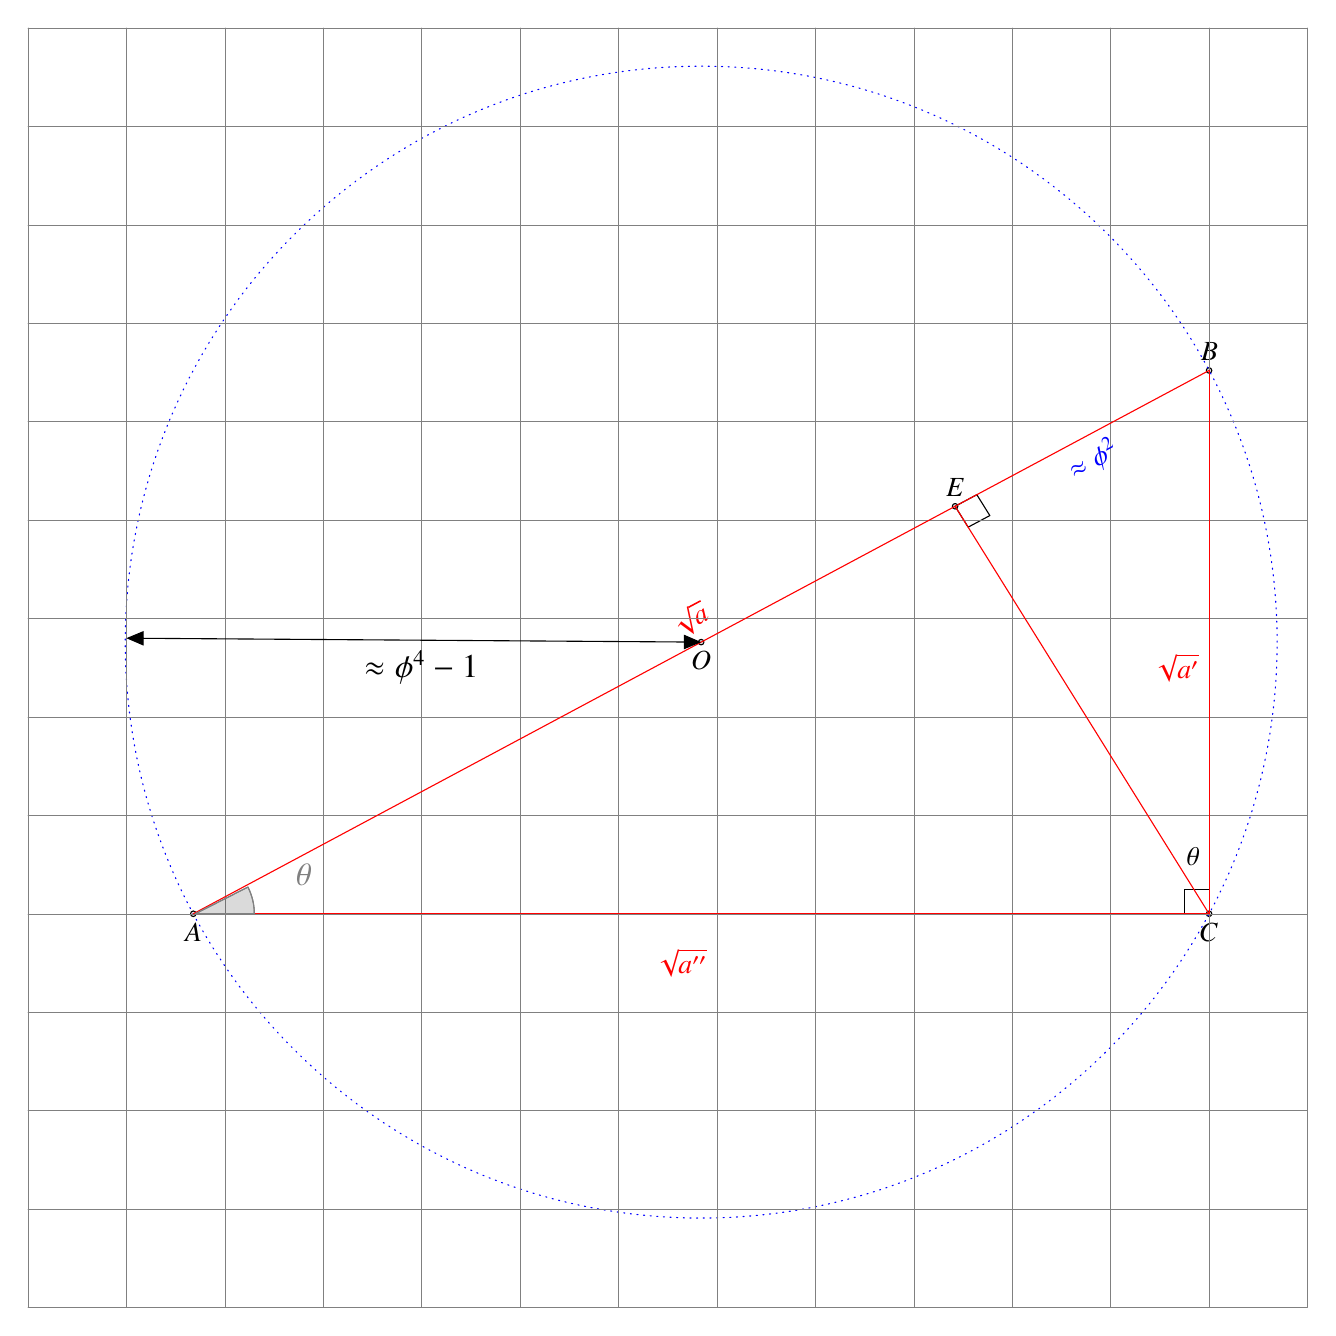
\begin{tikzpicture}[scale=1.25,line cap=round,line join=round,>=triangle 
45,x=1.0cm,y=1.0cm]
%\label{tab:13:table13}
\tkzDefPoint(-4.32,0.0){A} \tkzDefPoint(6.0,5.52){B} \tkzDefPoint(6.,0.){C} %\tkzDefPoint(0.0,0.0){D}
\tkzDrawPoints(A,B,C)
\tkzMarkRightAngle(B,C,A)
%\tkzMarkRightAngle(B,D,C)

\tkzLabelPoints[below](A,C)
\tkzLabelPoints[above](B)
\tkzDefMidPoint(A,B) \tkzGetPoint{O}
\coordinate (center) at (O);
\tkzLabelPoints[below](O)
\tkzDrawPoints(O)
%\tkzDefInterPoint(A,C) \tkzGetPoint{O}
\tkzLabelSegment[sloped,above,text=red](A,B){$\sqrt{a}$}
\draw[blue, dotted]
      let \p1 =  ($(-4.32,0)-(center)$),
          \n0 = {veclen(\x1,\y1)}
      in (center) circle(\n0);
\tkzDefMidPoint(O,B) \tkzGetPoint{E}
\tkzDrawPoints(E)
\tkzLabelPoints[above](E)
\tkzMarkRightAngle(B,E,C)
\draw[step=1cm,gray,very thin] (-6,-4) grid (7,9);
\draw[color=red] (-4.32,0.) -- (6.,0.);
\draw[color=red] (6.,0.) -- (6.,5.52);
\draw[color=red] (-4.32,0.) -- (6.,5.52);
\draw[color=red] (E) -- (C);
\tkzDefMidPoint(E,B) \tkzGetPoint{F}
\tkzLabelSegment[sloped,below,text=blue](E,B){$\approx \phi^{2}$}
%\tkzMarkAngle[fill=blue!20,size=0.4cm,opacity=.5](B,C,E)
\tkzLabelAngle[pos=0.6](B,C,E){$\theta$}
%\node [anchor = east] at (1.,3.5) {$\sqrt{a}$};
\node [anchor = east,text=red] at (6.,2.5) {$\sqrt{a'}$};
\node [anchor = east,text=red] at (1.,-0.5) {$\sqrt{a''}$};
\draw [<->] (O) node[left]{} -- (-5.0,2.8) node[right]{};
\clip(-6.,-0.4) rectangle (0.4,3.4);
\draw [shift={(-4.3,0.)},color=gray,fill=darkgray,fill opacity=0.1] (0,0) -- (0.:0.6) arc (0.:26.9:0.6) -- cycle;
\draw [shift={(-4.3,0.)},color=gray,fill=darkgray,fill opacity=0.1] (0,0) -- (0.:0.6) arc (0.:26.9:0.6) -- cycle;
%\draw[color=gray,fill=darkgray,fill opacity=0.1] (0.,0.42) -- (-0.42,0.42) -- (-0.42,0.) -- (0.,0.) -- cycle; 
%\draw (0.,6.)-- (-4.32,0.);
%\draw (6.,5.52)-- (-4.32,0.);
%\draw (6.,0.)-- (6.,5.52);
\draw[color=gray] (-3.2,0.4) node {\large $\theta$};
\draw[color=black] (-2.,2.5) node {\large $\approx \phi^4-1$};
\draw[color=gray] (0.34,0.33);
%\tkzMarkRightAngle[fill=blue!20](B,F,C)
\end{tikzpicture}
\caption{Electric Triangle properties.}
\end{figure}

\begin{figure}
\centering
\begin{tikzpicture}[scale=1.5,line cap=round,line join=round,>=triangle 
45,x=1.0cm,y=1.0cm]
%\label{tab:14:table14}
\draw[step=1cm,gray,very thin] (-3,-3) grid (6,6);
\tkzDefPoint(-1.42,0.0){A} \tkzDefPoint(5.,3.43){B} \tkzDefPoint(5.,0.){C} \tkzDefPoint(3.3,2.5){D}
\tkzDrawPoints(A,B,C,D)
\tkzMarkRightAngle(A,D,C)
\tkzLabelPoints[below](A,C)
\tkzLabelPoints[above](B,D)
\tkzMarkAngle[fill=blue!20,size=0.4cm,opacity=.5](C,A,B)
\tkzLabelAngle[pos=0.6](C,A,B){$\theta$}
\tkzDefMidPoint(A,B) \tkzGetPoint{O}
\coordinate (center) at (O);
\tkzLabelPoints[below](O)
\tkzDrawPoints(O)
\draw[blue, dotted]
      let \p1 =  ($(B)-(center)$),
          \n0 = {veclen(\x1,\y1)}
      in (center) circle(\n0);
\tkzMarkAngle[fill=blue!20,size=0.4cm,opacity=.5](B,C,D)
%\tkzMarkAngle[fill=blue!20,size=0.4cm,opacity=.5](O,E,D')
\tkzLabelAngle[pos=0.6](B,C,D){$\theta$}
\draw[color=red] (-1.42,0.) -- (5.,0.);
\draw[color=red] (5.,0.) -- (5.,3.43);
\draw[color=red] (-1.42,0.) -- (5.,3.43);
\draw[color=blue] (5.,0.) -- (3.3,2.5);
\node [anchor = east] at (3.9,1.0) {$q$};
\node [anchor = east] at (6.,1.5) {$q''$};
\node [anchor = east] at (2.5,-0.5) {$q'$};
\clip(-6.,-0.4) rectangle (0.4,3.4);
% 1st triangle


%\draw [shift={(-0.42,0.)},color=gray,fill=darkgray,fill opacity=0.1] (0,0) -- (0.:0.6) arc (0.:26.9:0.6) -- cycle;
%\draw[color=gray,fill=darkgray,fill opacity=0.1] (0.,0.42) -- (-0.42,0.42) -- (-0.42,0.) -- (0.,0.) -- cycle; 
%\draw (0.,6.)-- (-4.32,0.);
%\draw (6.,5.52)-- (-4.32,0.);
%\draw (6.,0.)-- (6.,5.52);
%\draw[color=gray] (0.,0.8) node {\large $\theta$};
%\draw[color=gray] (0.34,0.33);
%\tkzMarkRightAngle[fill=blue!20](B,F,C)
\end{tikzpicture}
\caption{Weinberg Triangle properties.}
\end{figure}

\begin{figure}
\centering
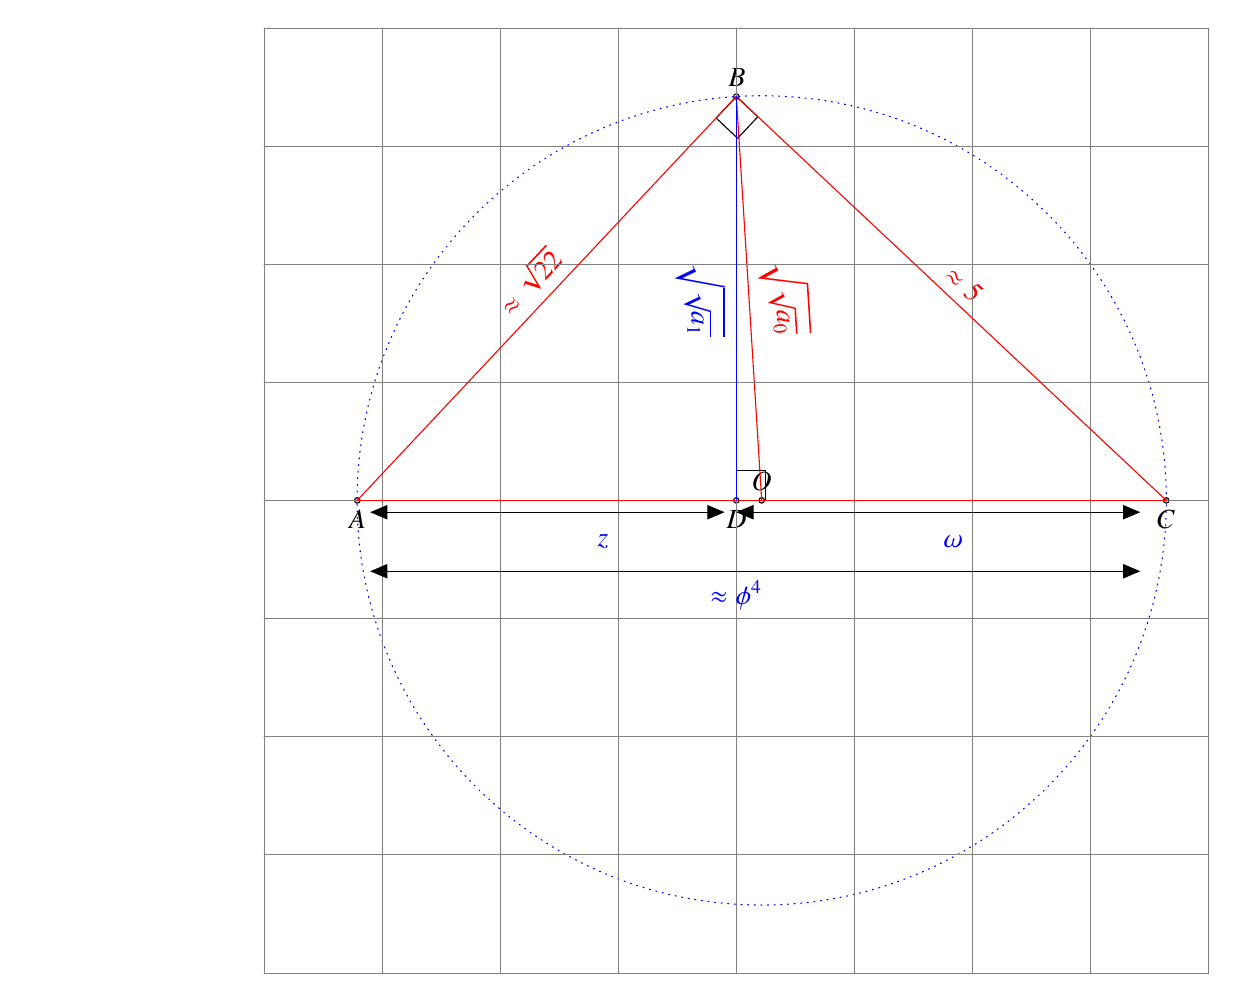
\begin{tikzpicture}[scale=1.5,line cap=round,line join=round,>=triangle 
45,x=1.0cm,y=1.0cm]
%\label{tab:15:table15}
\tkzDefPoint(-3.21,0.0){A} \tkzDefPoint(0.0,3.42){B} \tkzDefPoint(3.64,0.){C} \tkzDefPoint(0.0,0.0){D}
\tkzDrawPoints(A,B,C,D)
\tkzMarkRightAngle(A,B,C)
\tkzMarkRightAngle(B,D,C)
\tkzLabelPoints[below](A,C,D)
\tkzLabelPoints[above](B)
%\tkzMarkAngle[fill=blue!40,size=1.4cm,opacity=.5](C,A,B)
%\tkzLabelAngle[pos=1.6](C,A,B){$\theta$}
\tkzDefMidPoint(A,C) \tkzGetPoint{O}
\coordinate (center) at (O);
\tkzLabelPoints[above](O)
\tkzDrawPoints(O)
\tkzLabelSegment[sloped,above,text=red](A,B){$\approx \sqrt{22}$}
\tkzLabelSegment[sloped,above,text=red](B,C){$\approx 5$}
%\tkzLabelSegment[sloped,below,text=red](A,C){$\approx \phi^{4}$}
\draw[blue, dotted]
      let \p1 =  ($(B)-(center)$),
          \n0 = {veclen(\x1,\y1)}
      in (center) circle(\n0);
\draw[color=red] (B) -- (O);
\tkzDefMidPoint(B,O) \tkzGetPoint{F}
\tkzLabelSegment[sloped,above,text=red](B,O){$\sqrt{\sqrt{a_0}}$}
\draw[color=blue] (B) -- (D);
\tkzDefMidPoint(B,D) \tkzGetPoint{G}
\tkzLabelSegment[sloped,below,text=blue](B,D){$\sqrt{\sqrt{a_1}}$}
\draw[step=1cm,gray,very thin] (-4,-4) grid (4,4);
\draw[color=red] (-3.21,0.) -- (0.,0.);
\draw[color=red] (3.64,0.) -- (0.,0.0);
\draw[color=red] (-3.21,0.) -- (0.,3.42);
\draw[color=red] (0.,3.42) -- (3.64,0.);
\draw[color=blue] (0.,0.) -- (0.,3.42);
%\node [anchor = east] at (0.,1.5) {$\sqrt{\sqrt{a_1}}$};
%\node [anchor = east] at (2.,2.0) {$\approx 5$};
%\node [anchor = east] at (-1.,2.0) {$\approx \sqrt{22}$};
\node [anchor = north,text=blue] at (0.,-0.6) {$\approx \phi^{4}$};
\draw [<->] (-3.1,-0.1) node[left]{} -- (-0.1,-0.1) node[right]{};
\draw [<->] (0.0,-0.1) node[left]{} -- (3.42,-0.1) node[right]{};
\draw [<->] (-3.1,-0.6) node[left]{} -- (3.42,-0.6) node[right]{};
  %\draw [decoration={markings,mark=at position 1 with
   % {\arrow[scale=3,>=stealth reversed]{<}}},postaction={decorate}] (-3.2,-0.3) -- (3.42,-0.3);
\node [anchor = east,text=blue] at (2.,-0.35) {$\omega$};
\node [anchor = east,text=blue] at (-1.,-0.35) {$z$};
\clip(-6.,-0.4) rectangle (0.4,3.4);
%\draw [shift={(-3.2,0.)},color=gray,fill=darkgray,fill opacity=0.1] (0,0) -- (0.:0.6) arc (0.:43.9:0.6) -- cycle;
%\draw[color=gray,fill=darkgray,fill opacity=0.1] (0.,0.42) -- (-0.42,0.42) -- (-0.42,0.) -- (0.,0.) -- cycle; 
%\draw (0.,6.)-- (-4.32,0.);
%\draw (6.,5.52)-- (-4.32,0.);
%\draw (6.,0.)-- (6.,5.52);
%\draw[color=gray] (-3.2,0.4) node {\large $\theta$};
%\draw[color=gray] (0.34,0.33);
%\tkzMarkRightAngle[fill=blue!20](B,F,C)
\end{tikzpicture}
\caption[The Golden Sanchez Triangle properties.]{Golden Sanchez Triangle.}
\end{figure}

\begin{figure}
\centering
\begin{tikzpicture}[scale=1.75, line cap=round,line join=round,>=triangle 
45,x=1.0cm,y=1.0cm]
%\label{tab:15:table15}
\tkzDefPoint(-0.236,0.0){A} \tkzDefPoint(0.0,0.944){B} \tkzDefPoint(3.764,0.){C} \tkzDefPoint(0.0,0.0){D} \tkzDefPoint(0.882,0.0){D'} \tkzDefPoint(0.882,-1.764){E}
\tkzDrawPoints(A,B,C,D,D',E)
\tkzMarkRightAngle(A,B,C)
\tkzMarkRightAngle(B,D,C)
\tkzMarkRightAngle(E,D',C)
\tkzMarkRightAngle(A,E,C)
\tkzLabelPoints[below](A,C,D,E)
\tkzLabelPoints[above](B,D')
\tkzDefMidPoint(A,C) \tkzGetPoint{O}
\coordinate (center) at (O);
\tkzLabelPoints[below](O)
\tkzDrawPoints(O)
\tkzMarkAngle[fill=blue!20,size=0.4cm,opacity=.5](B,O,D)
%\tkzMarkAngle[fill=blue!20,size=0.4cm,opacity=.5](O,E,D')
\tkzLabelAngle[pos=0.6](B,O,D){$\theta$}
\tkzLabelAngle[pos=0.6](O,E,D'){$\theta$}
%\tkzMarkAngle[fill=blue!40,size=1.4cm,opacity=.5](C,A,B)
%\tkzLabelAngle[pos=1.6](C,A,B){$\theta$}
\draw[step=1cm,gray,very thin] (-1,-3) grid (4,3);

\draw[color=green] (-0.236,0.) -- (0.882,-1.764);
%\draw[color=green] (-1.764,0.) -- (0.,0.0);
\draw[color=green] (-0.236,0.) -- (3.826,0.);
\draw[color=green] (0.882,-1.764) -- (3.826,0.);
\draw[color=blue] (0.882,0.) -- (0.882,-1.764);
% 1st triangle
\draw[color=red] (-0.236,0.) -- (0.,0.944);
\draw[color=red] (0.944,0.) -- (0.,0.0);
\draw[color=red] (-0.236,0.) -- (3.764,0.);
\draw[color=red] (0.,0.944) -- (3.764,0.);
\draw[color=blue] (0.,0.) -- (0.,0.944);
\draw[color=blue] (B) -- (O);
\draw[color=blue] (E) -- (O);
\draw[blue, dotted]
      let \p1 =  ($(-0.236,0)-(center)$),
          \n0 = {veclen(\x1,\y1)}
      in (center) circle(\n0);


%\node [anchor = east] at (0.,1.5) {$h$};
%\node [anchor = east] at (2.,2.0) {$\approx 5$};
%\node [anchor = east] at (-1.,2.0) {$\approx \sqrt{22}$};
%\node [anchor = north] at (0.,-0.7) {$\approx \phi^{4}$};
%\draw [<->] (-3.1,-0.1) node[left]{} -- (-0.2,-0.1) node[right]{};
%\draw [<->] (0.2,-0.1) node[left]{} -- (3.42,-0.1) node[right]{};
%\draw [<->] (-3.1,-0.6) node[left]{} -- (3.42,-0.6) node[right]{};
  %\draw [decoration={markings,mark=at position 1 with
   % {\arrow[scale=3,>=stealth reversed]{<}}},postaction={decorate}] (-3.2,-0.3) -- (3.42,-0.3);
%\node [anchor = east] at (2.,-0.35) {$\omega$};
%\node [anchor = east] at (-1.,-0.35) {$z$};
\clip(-6.,-0.4) rectangle (0.4,3.4);
%\draw [shift={(-3.2,0.)},color=gray,fill=darkgray,fill opacity=0.1] (0,0) -- (0.:0.6) arc (0.:43.9:0.6) -- cycle;
%\draw[color=gray,fill=darkgray,fill opacity=0.1] (0.,0.42) -- (-0.42,0.42) -- (-0.42,0.) -- (0.,0.) -- cycle; 
%\draw (0.,6.)-- (-4.32,0.);
%\draw (6.,5.52)-- (-4.32,0.);
%\draw (6.,0.)-- (6.,5.52);
%\draw[color=gray] (-3.2,0.4) node {\large $\theta$};
%\draw[color=gray] (0.34,0.33);
%\tkzMarkRightAngle[fill=blue!20](B,F,C)
\end{tikzpicture}
\caption[The holographic Triangle properties.]{Holographic triangle is caracterized by $S=h=\sin\theta$; the height h and the area S are both equal to $\sin\theta$.}
\end{figure}


\begin{figure}
\centering
\begin{tikzpicture}
%\tkzInit[xmax=6.4, zmax=3.4]
\tkzDefPoint(0.0,0.0){A} \tkzDefPoint(6.4,0.0){B} \tkzDefPoint(5.1,-1.3){C} \tkzDefPoint(4.0,-1.0){q}
\tkzDrawPoints(A,B,C,q)
\tkzDefMidPoint(B,q) \tkzGetPoint{D}
%\tkzDefPoint[label={[align=left]right:$q$},xshift=00mm](4.5,-0.5){D}
\tkzLabelSegment[sloped,text=red,xshift=-06mm](q,B){$q$}
\tkzMarkRightAngle(A,B,C)
\tkzMarkRightAngle(B,q,C)
\tkzLabelPoints[below](A,B,C)
%\tkzLabelPoints[above right](q)
\tkzMarkAngle[fill=blue!40,size=1.4cm,opacity=.5](C,A,B)
\tkzLabelAngle[pos=1.6](C,A,B){$\theta$}
    %\draw [important line] (0.0,0.) coordinate (A) -- (5.1,-1.3) coordinate (C) node[below, text width=5em] {}
    %\draw [blue] (6.4,0.) coordinate (A) -- (4.,-1.0) coordinate (D) node[below, text width=5em] {$h$}
    %\draw [red] (6.4,0.) coordinate (B) -- (4.,-1.0) coordinate (D) node[below, text width=5em] {$q$}
  \draw (6.4,0,0) coordinate (x) |- (0,10,0) coordinate [midway] (h) coordinate (y) -- (0,10,3.4) coordinate (a) -- (0,0,3.4) coordinate (z) -- (6.4,0,3.4) edge (x) -- (6.4,10,3.4) coordinate (v) edge (h)
  -- (a)  ;
  \draw [dashed] (0,0,0) coordinate (o) edge (x) edge (y) -- (z);
  \draw [dashed] (0,0,0) coordinate (o) edge (x) edge (v) -- (v);
  \draw [blue] (0,0,0)  -- (6.4,0.0,3.4);
  \draw [red] (4.9,0.02,2.7)  -- (6.4,0.0,0.0);
  %\node [circle, minimum size=2pt, inner sep=0pt, fill, label=135:$\sqrt{2a^3/pp_G}$] at (v) {};
  \draw [very thin,black,line join=round] (0,0,0)  -- node [sloped,above] {$\sqrt{2a^3/pp_G}$} (6.4,10,3.4);
  \node [circle, minimum size=4pt, inner sep=0pt, fill, label=135:o] at (o) {};
  \draw [decoration={markings,mark=at position 1 with
    {\arrow[scale=3,>=stealth]{>}}},postaction={decorate}] (0,0,0) -- (6.4,10,3.4);
  \draw [dashed] (0,0,0) -- (6.4,0,3.4);
  \draw [->] (x) -- +(3pt,0,0) node [midway,above] {$q'$};
  \draw [->] (y) -- +(0,3pt,0) node [midway,right] {$1$};
  \draw [->] (z) -- +(0,0,3pt) node [midway,above] {$q''$};
  %\draw (v) -- ++(0,0,-2) coordinate (d) -- ++(-2,0,0) coordinate (e) -- ++(0,0,2) |- ++(2,-2,0) coordinate [midway] (f) -- ++(0,0,-2) coordinate (g) -- (d);
  %\draw [dashed] (e) -- ++(0,-2,0) coordinate (c) edge (f) -- (g);
  %\node [label=45:C] at (c) {};
  %\draw[red]   (0,0,0) -- (.95,0,0)    node[red,left=6pt]    {$x$};
\end{tikzpicture}
\caption[The Weinberg-Sanchez cuboid properties]{3D perspective of the "Weinberg-Sanchez" cuboid: Electro-weak / Gravitation connection}
\end{figure}

\begin{figure}
\centering
\begin{tikzpicture}[scale=1.25]
%\tkzInit[xmax=6.4, zmax=3.4]
\tkzDefPoint(0.0,0.0){C} \tkzDefPoint(4.9,0.0){B} \tkzDefPoint(3.12,-1.74){A} \tkzDefPoint(1.8,-1.0){q}
\tkzDrawPoints(A,B,C,q)
\tkzDefMidPoint(B,q) \tkzGetPoint{D}
%\tkzDefPoint[label={[text=blue,align=left]right:$z$},xshift=-01mm](2.25,-1.50){F}
%\tkzDefPoint[label={[text=blue,align=left]right:$\omega$},xshift=-01mm](0.75,-0.70){E}
%\tkzDefPoint[label={[text=red,align=left]right:$\sqrt{\omega z}$},xshift=-01mm](2.8,-0.29){D}
%\tkzDefPoint[label={[align=right]right:$4 \cdot \sqrt{(3H\beta/n)}$},xshift=00mm](3.0,-0.79){D}
\tkzLabelSegment[sloped,below,text=red](q,B){$\sqrt{\omega z}$}
\tkzLabelSegment[sloped,below,text=blue](A,q){$z$}
\tkzLabelSegment[sloped,below,text=blue](C,q){$\omega$}
\tkzLabelSegment[sloped,text=blue,xshift=1.5mm,yshift=-07.5mm](A,C){$\phi^4$}
\tkzMarkRightAngle(A,B,C)
\tkzMarkRightAngle(B,q,C)
\tkzLabelPoints[below](A,B,C)
\tkzDrawSegments[red](B,q)
%\tkzLabelPoints[above right](q)
%\tkzMarkAngle[fill=blue!40,size=1.4cm,opacity=.5](C,A,B)
%\tkzLabelAngle[pos=0.6](A,q,B){$\sqrt{\omega z}$}
    %\draw [important line] (0.0,0.) coordinate (A) -- (5.1,-1.3) coordinate (C) node[below, text width=5em] {}
    %\draw [blue] (6.4,0.) coordinate (A) -- (4.,-1.0) coordinate (D) node[below, text width=5em] {$h$}
    %\draw [red] (6.4,0.) coordinate (B) -- (4.,-1.0) coordinate (D) node[below, text width=5em] {$q$}
  \draw (4.9,0,0) coordinate (x) |- (0,1,0) coordinate [midway] (h) coordinate (y) -- (0,1,4.6) coordinate (a) -- (0,0,4.6) coordinate (z) -- (4.9,0,4.6) edge (x) -- (4.9,1,4.6) coordinate (v) edge (h)
  -- (a)  ;
  \draw [dashed] (0,0,0) coordinate (o) edge (x) edge (y) -- (z);
  \draw [dashed] (0,0,0) coordinate (o) edge (x) edge (v) -- (v);
  \draw [blue] (0,0,0)  -- (4.9,0.0,4.6);
  \draw [very thin,black,line join=round] (0,0,0)  -- node [sloped,above,xshift=-0.mm,yshift=-2.mm] {$4\sqrt{(3H\beta/n)}$} (4.9,1.,4.6);
  %\node [circle, minimum size=2pt, inner sep=0pt, fill, label=135:$4 \cdot \sqrt{(3H\beta/n)}$] at (v) {};
  \node [circle, minimum size=4pt, inner sep=0pt, fill, label=135:o] at (o) {};
  \draw [decoration={markings,mark=at position 1 with
    {\arrow[scale=3,>=stealth]{>}}},postaction={decorate}] (0,0,0) -- (4.9,1,4.6);
  %\draw [<->] (0.2,-0.5) node[left]{} -- (2.2,-1.8) node[below]{$\phi^4$};
  \draw [->] (x) -- +(3pt,0,0) node [midway,above] {$\sqrt{\omega \cdot (\omega+z)}$};
  \draw [->] (y) -- +(0,3pt,0) node [midway,right] {$1$};
  \draw [->] (z) -- +(0,0,3pt) node [midway,above] {$\sqrt{z \cdot (\omega+z)}$};
  %\draw (v) -- ++(0,0,-2) coordinate (d) -- ++(-2,0,0) coordinate (e) -- ++(0,0,2) |- ++(2,-2,0) coordinate [midway] (f) -- ++(0,0,-2) coordinate (g) -- (d);
  %\draw [dashed] (e) -- ++(0,-2,0) coordinate (c) edge (f) -- (g);
  %\node [label=45:C] at (c) {};
  %\draw[red]   (0,0,0) -- (.95,0,0)    node[red,left=6pt]    {$x$};
\end{tikzpicture}
\caption[The Golden Sanchez cuboid properties]{3D perspective of the "Golden-Sanchez" cuboid: Electro-weak / Eddington matrix connection}
\end{figure}

\end{appendix}

\end{document}
